\documentclass{acm_proc_article-sp}
\usepackage[utf8]{inputenc}
\usepackage{ucs}
\usepackage[brazil]{babel}
\usepackage[T1]{fontenc}
\usepackage{url}
\usepackage{amsmath}
\usepackage{multirow}
\usepackage{amssymb}
\author{Felipe Pereira Coelho}
\usepackage{cite}
\usepackage{graphicx}
\graphicspath{{img/}}
\DeclareGraphicsExtensions{.pdf,.png,.jpg,.gif}
\usepackage{amsmath}
\usepackage[titletoc,toc,page]{appendix}
\renewcommand{\appendixtocname}{Ap\'endices}
\renewcommand{\appendixpagename}{Ap\'endices}

\begin{document}

\title{ T-AADSP - Uma ferramenta de apoio a implantação adaptativa de processo de software}

\numberofauthors{2} 
\author{
% You can go ahead and credit any number of authors here,
% e.g. one 'row of three' or two rows (consisting of one row of three
% and a second row of one, two or three).
%
% The command \alignauthor (no curly braces needed) should
% precede each author name, affiliation/snail-mail address and
% e-mail address. Additionally, tag each line of
% affiliation/address with \affaddr, and tag the
% e-mail address with \email.
%
% 1st. author
\alignauthor
Felipe Pereira Coelho\ \\
       \affaddr{Instituto Federal de Educação, Ciência e Tecnologia da Bahia}\\
       \affaddr{Rua Emídio dos Santos, S/N, Barbalho}\\
       \affaddr{Salvador, Bahia}\\
       \email{felipecoelho@ifba.edu.br}
% 2nd. author
\alignauthor
Antonio Carlos Santos Souza\ \\
       \affaddr{Instituto Federal de Educação, Ciência e Tecnologia da Bahia}\\
       \affaddr{Rua Emídio dos Santos, S/N, Barbalho}\\
       \affaddr{Salvador, Bahia}\\
       \email{antoniocarlos@ifba.edu.br}
}


\maketitle
\begin{abstract}
As abordagens existentes para o gerenciamento de projetos de \textit{software} não são fáceis de serem implementadas nas empresas. Neste projeto, será proposta uma ferramenta baseada na metodologia para gerenciamento de projetos de \textit{software} \textit{AADSP}, metodologia esta que utiliza conceitos das abordagens ágeis, preservando as práticas consideradas como relevantes ao cenário de desenvolvimento de \textit{software} e as abordagens não ágeis, que definem diversos processos e resultados esperados pelas mais diversas fases e atividades de um projeto. 
\end{abstract}

\keywords{Engenharia de \textit{Software}, Artefatos de \textit{Software}, Gerenciamento de Projetos de \textit{Software}} % NOT required for Proceedings



\section{Introdução}
No século XXI o desenvolvimento de software tem adquirido bastante força e movimentando um mercado bilionário de aplicativos e softwares dos mais diversos nichos. Para prover maior potencialização no desenvolvimento de software, a indústria tem recorrido a área da engenharia de software. Esta área vem buscando solucionar a questão de se desenvolver softwares de forma rápida, com baixo custo e alta qualidade. Nesta constante busca, a área da engenharia de software têm desenvolvido técnicas e estudos de processos em diversos cenários de desenvolvimento.

O primeiro modelo de desenvolvimento de software foi denominado de clássico ou cascata, que também é conhecido por abordagem “top-down”. Este proposto por Royce em 1970 \cite{Royce}. Até meados da década de 1980, foi o único modelo com aceitação geral. Este modelo segmentava o processo de desenvolvimento de software em fases. Estas eram compostas em: requerimento, projeto, implementação, verificação e manutenção. Em cada uma das fases mencionadas eram esperados um conjunto de resultados, ao término de uma determinada fase o projeto seguia para uma conseguinte não sendo admitido retorno a uma fase anterior já executada. O grande problema do modelo é que projetos, em especial os de software, sofrem constante mudança no decorrer de sua execução, porem isto não era previsto pelo modelo o tornando difícil de ser implementado.

Outros métodos baseados na abordagem clássica surgiram e são denominados de métodos tradicionais, estes são altamente prescritivos e, de forma geral, se caracterizam pelo foco em planos detalhados definidos no princípio do projeto. Acreditava-se que, pelo uso desses métodos, seria possível tratar o desenvolvimento de \textit{software} como um processo previsível, no
que, quanto mais falhavam, mais pesados e complexos esses métodos se tornavam \cite{scrum:agil}.

Para que se tenha um setor de \textit{software} competitivo, nacional e internacionalmente, é essencial que os empreendedores do setor coloquem a eficiência e a eficácia dos seus processos em foco nas empresas,
visando à oferta de produtos de \textit{software} e serviços correlatos, conforme padrões internacionais de qualidade \cite{mpsbr:nAgil}. Nesse contexto, surgem diversas metodologias que visam promover a implantação e a melhoria contínua do processo de \textit{software} nas empresas. Neste cenário, a qualidade dos produtos tem se tornado um fator diferencial e está diretamente ligada ao processo utilizado para conceber os mesmos. Um processo é uma sequencia de passos realizados para um determinado propósito \cite{ieee}. Um processo de \textit{software} é definido como um conjunto de atividades, métodos, práticas e transformações que pessoas empregam para desenvolver e manter \textit{software} e produtos associados \cite{weber}. O Guia Brasileiro de Melhoria de Processo de \textit{Software} - MPSBR define que qualidade é um fator crítico para o sucesso
da indústria de \textit{software}. 

\section{Fundamentação teórica}
Durante o processo de concepção do presente trabalho, foi necessária a realização de uma revisão da literatura com o objetivo de levantar a fundamentação teórica ao tema proposto. Nesta seção, serão apresentados os principais temas encontrados e utilizados no desenvolvimento deste trabalho, que será fundamentado no manifesto ágil de desenvolvimento de \textit{software} \cite{manifesto:agil} e alguns guias de melhoria de processo de \textit{software}. Desse modo, será realizada a separação dos temas analisados em três categorias:

\begin{itemize}
\item Abordagens ágeis,
\item Abordagens não ágeis, e
\item Abordagens híbridas.
\end{itemize}

Para classificarmos as abordagens adotaremos o seguinte: 

\begin{enumerate}
\item  Neste trabalho, serão consideradas abordagens ágeis aquelas que estiverem de acordo com o manifesto ágil de \textit{software}. Essa classificação será dada independentemente da classificação originalmente atribuída pelos autores de cada abordagem;
\item Para abordagens não ágeis adotaremos esta classificação, a medida que, o autor focar seus processos em documentos e descartar ou minimizar os valores e princípios definidos no manifesto ágil de \textit{software};
\item Será considerada uma abordagem como híbrida, quando o próprio autor fizer esta afirmativa ou quando esta abordagem estiver relacionando seus processos e documentos aos princípios e valores do manifesto ágil de maneira valorativa aos documentos e processos.
\end{enumerate}

\subsection{Abordagens ágeis}

\subsubsection{SCRUM}
O \textit{Scrum} é definido como uma metodologia ágil para gestão e planejamento de projetos de software \cite{scrum:agil}.

Utilizando esta metodologia de desenvolvimento \textit{Scrum}, os projetos devem ser dividos em ciclos (tipicamente mensais) chamados de \textit{Sprints}. O \textit{Sprint} representa um \textit{Time Box} dentro do qual um conjunto de atividades ,previamente levantadas, serão executadas. Metodologias ágeis de desenvolvimento de \textit{software} são iterativas, ou seja, o trabalho é dividido em iterações, que são chamadas de \textit{Sprints} \cite{scrum:agil}. No caso do \textit{Scrum}, as funcionalidades a serem implementadas em um projeto são mantidas em uma lista. Esta é conhecida como \textit{Product Backlog} e no início de cada \textit{Sprint} faz-se um \textit{Sprint Planning Meeting}, ou seja, uma reunião de planejamento na qual o \textit{Product Owner} prioriza os itens do \textit{Product Backlog} e a equipe seleciona as atividades que ela será capaz de implementar durante o \textit{Sprint} que se inicia. Assim, as tarefas alocadas em um \textit{Sprint} são transferidas do \textit{Product Backlog} para o \textit{Sprint Backlog} \cite{scrum:agil}.

A cada dia do \textit{Sprint} em execução, a equipe faz uma breve reunião (normalmente de manhã), chamada \textit{Daily Scrum}. A reunião mencionada objetiva disseminar conhecimento sobre o que foi feito no dia anterior, realizar a identificação dos impedimentos e priorizar o trabalho do dia que se inicia \cite{scrum:agil}. Ao final de um \textit{Sprint}, a equipe apresenta as funcionalidades implementadas em uma \textit{Sprint Review Meeting}. Finalmente, faz-se uma \textit{Sprint Retrospective} e a equipe parte para o planejamento do próximo \textit{Sprint} \cite{scrum:agil}.

Papéis definidos no \textit{Scrum}

\begin{itemize}
\item \textbf{Product Owner:}  O \textit{Product Backlog} é uma lista contendo todas as funcionalidades desejadas para um produto. O conteúdo desta lista é definido pelo \textit{Product Owner} \cite{scrum:agil}.
\item \textbf{Scrum Master:} O \textit{Scrum Master} procura assegurar que a equipe respeite e siga os valores e as práticas do \textit{Scrum}. Ele também protege a equipe assegurando que ela não se comprometa excessivamente com relação àquilo que é capaz de realizar durante um \textit{Sprint} \cite{scrum:agil}.
\item \textbf{Scrum Team:} O \textit{Scrum Team} é a equipe de desenvolvimento. Nela, não existe necessariamente uma divisão funcional através de papéis tradicionais, tais como: programador, designer, analista de testes ou arquiteto. Todos no projeto trabalham juntos para completar o conjunto de trabalho com o qual se comprometeram conjuntamente para um \textit{Sprint} \cite{scrum:agil}.
\end{itemize}


\begin{figure}[h]
\centering % para centralizarmos a figura
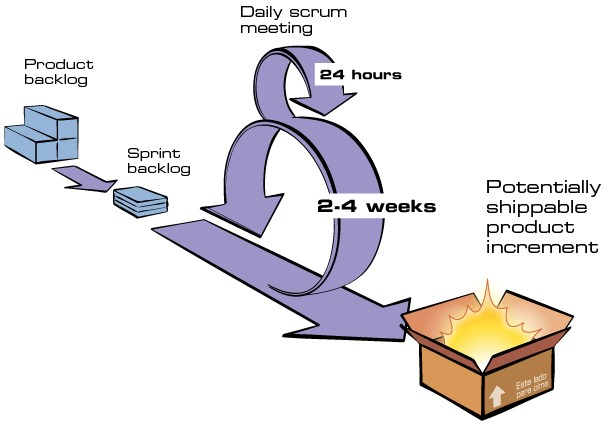
\includegraphics[width=0.5\textwidth]{scrumCiclo.JPG} % leia abaixo
\caption{Ciclos do \textit{Scrum} \cite{scrum:agil}}
\end{figure}


\subsubsection{XP}
\textit{Extreme Programming (XP)} é uma metodologia de desenvolvimento de \textit{software}, nascida nos Estados Unidos ao final da década de 90. Esta metodologia possui exito em diversos países, por ajudar a criar sistemas de melhor qualidade, que são produzidos em menor tempo e de forma mais econômica que o habitual. Tais objetivos são alcançados através de um pequeno conjunto de valores, princípios e práticas, que diferem substancialmente da forma tradicional de se desenvolver \textit{software} \cite{xp:agil}.

O XP divide os valores em:

\begin{itemize}
\item \textbf{Comunicação:} Embora existam inúmeras formas de se comunicar ideias, algumas são mais eficazes que outras. Por exemplo, quando duas pessoas estabelecem um diálogo presencial, inúmeros elementos da comunicação colaboram para a compreensão do assunto, tais como: gestos, expressões faciais, postura, palavras verbalizadas, tom de voz, emoções, entre outros. Quanto maior a capacidade de compreensão, maiores as chances de evitar problemas como: ambiguidades, entendimento equivocados, entre outros\cite{xp:agil}.
\item \textbf{Coragem:} Equipes XP confiam na eficácia destas práticas e destes mecanismos de proteção e isso é o que as tornam receptivas a mudanças. Assim, ao invés de frear a criatividade do cliente e evitar mudanças, equipes XP as consideram inevitáveis e procuram se adaptar a elas com segurança e com coragem, isto é, com confiança em seus mecanismos de proteção, tais como: desenvolvimento orientado a testes, programação em par e integração contínua \cite{xp:agil}.
\item \textbf{Feedback:} Projetos XP estabelecem formas de encurtar ao máximo a defasagem de tempo entre o momento em que uma ação é executada e seu resultado. Assim, por exemplo, desenvolvedores procuram entregar novas funcionalidades no menor prazo possível, para que o cliente compreenda rapidamente as conseqüências daquilo que pediu \cite{xp:agil}.
\item \textbf{Respeito:} Respeito é um valor que dá sustentação a todos os demais.Os integrantes de uma equipe só irão se preocupar em comunicar-se melhor, por exemplo, se se importarem uns com os outros. O respeito é base de todos os valores. Se ele não existir em um projeto, não há nada que possa salvá-lo. Saber ouvir, saber compreender e respeitar o ponto de vista do outro é essencial para que um projeto de \textit{software} seja bem sucedido \cite{xp:agil}.
\item \textbf{Simplicidade:} o conceito de simplicidade, em inúmeros aspectos do projeto, assegura que a equipe se concentre em fazer, apenas aquilo que é claramente necessário e evite fazer o que poderia vir a ser necessário, mas ainda não se provou essencial \cite{xp:agil}.
\end{itemize}

\subsection{Abordagens não Ágeis}
\subsubsection{Implantação e gerenciamento de processos com PMBOK}
Nesta secção, iremos dar enfoque ao processo de gerenciamento de projetos definidos pelo Guia PMBOK. O Guia do Conhecimento em Gerenciamento de Projeto (Guia PMBOK) foi desenvolvido pelo PMI (\textit{Project Management Institute}), sendo mantido pela mesma instituição desenvolvedora do Guia. O Guia PMBOK fornece diretrizes para o gerenciamento de projetos individuais e define os conceitos relacionados com o gerenciamento de projetos. Ele também descreve o ciclo de vida de gerenciamento e seus respectivos processos, assim como o ciclo de vida do projeto \cite{pmbok:nAgil}. A partir deste momento, quando nos referirmos ao Guia do Conhecimento em Gerenciamento de Projeto, adotaremos a conotação ao mesmo de Guia PMBOK.

Segundo o Guia PMBOK, o gerenciamento de projetos é a aplicação do conhecimento, das habilidades, das ferramentas e das técnicas às atividades do projeto para atender aos seus requisitos. O gerenciamento de projetos é realizado através da aplicação e integração apropriadas dos quarenta e sete processos de gerenciamento de projetos, logicamente agrupados em cinco grupos de processos \cite{pmbok:nAgil}, conforme descritos a seguir:

%Lista de itens
\begin{itemize}
\item Iniciação;
\item Planejamento;
\item Execução;
\item Monitoramento e controle;
\item Encerramento.
\end{itemize}

Para o Guia PMBOK, no processo de gerenciamento de um projeto, normalmente se inclui mas não se limita: a identificação dos requisitos, abordagem das diferentes necessidades, preocupações e expectativas das partes interessadas no planejamento e execução do projeto, o estabelecimento e manutenção e execução de comunicações ativas, eficazes e colaborativas entre as partes interessadas, a realização do gerenciamento das partes interessadas visando o atendimento aos requisitos do projetos e a criação de suas entregas \cite{pmbok:nAgil}. Devendo ser realizado também um equilíbrio das restrições conflitantes de um projeto que incluem:

%Lista de itens
\begin{itemize}
\item Escopo;
\item Qualidade;
\item Cronograma;
\item Orçamento;
\item Recursos e 
\item Riscos.
\end{itemize}

O Guia PMBOK descreve que os fatores mencionados estão relacionados de tal forma que se algum deles mudar, pelo menos um outro fator será afetado \cite{pmbok:nAgil}. Será apresentado a seguir o detalhamento das restrições conflitantes de um projeto, pelo fato destas serem consideradas um fator crucial ao processo de implantação e gerenciamento de um projeto de software.  

\subsubsection*{Escopo}
Para planejar o gerenciamento do escopo deve ser confeccionado um plano onde ser documentada sua definição, validade e controle. O principal objetivo deste processo é o fornecimento de orientações e instruções sobre como o escopo será gerenciado ao longo de todo o projeto.

A figura abaixo ilustra o que deverá ser realizado:

\begin{figure}[h]
\centering % para centralizarmos a figura
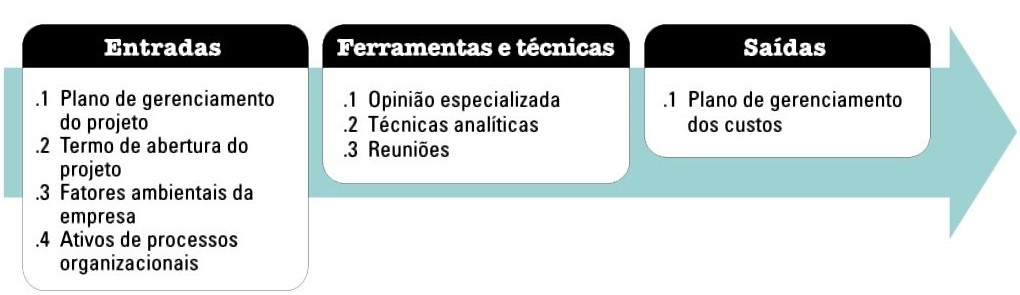
\includegraphics[width=0.5\textwidth]{entradaescopo.jpg} % leia abaixo
\caption{Fluxo do processo: Entradas, ferramentas, técnicas e saídas \cite{pmbok:nAgil}}
\end{figure}

Nesta etapa são definidos alguns artefatos do projeto como: plano de gerenciamento, o termo de abertura e discriminação dos fatores ambientais da empresa que consiste em:

\begin{itemize}
\item Cultura Organizacional;
\item Infraestrutura;
\item Administração do Pessoal e
\item Condições de Mercado.
\end{itemize} 

Além disso, o  Guia PMBOK inclui nesta fase a definição de processos organizacionais onde deve ser incluso as:

\begin{itemize}
\item Políticas e procedimentos, e
\item Informações históricas e base de conhecimento de lições aprendidas
\end{itemize}

No âmbito das ferramentas e técnicas, deverá ser consultada uma opinião especializada que consiste em entradas recebidas das partes entendidas e experientes \cite{pmbok:nAgil}. O Guia PMBOK define que para as reuniões, a equipe do projeto poderá participar das mesmas e promover a definição do plano de gerenciamento do escopo do projeto.

No que se refere as saídas, deverá ser desenvolvido o plano de gerenciamento do escopo do projeto, este que é um componente do plano de gerenciamento do projeto ou do programa que descreve como escopo será definido, desenvolvido, monitorado, controlado e verificado \cite{pmbok:nAgil}.

O plano de gerenciamento dos requisitos é definido pelo Guia PMBOK como um componente do plano de gerenciamento do projeto, este descreve como os requisitos serão analisados, documentados e gerenciados. 

\subsubsection*{Qualidade}
O gerenciamento da qualidade do projeto inclui os processos e as atividades da organização executora que determinam as políticas de qualidade, os objetivos e as responsabilidades, de modo que o projeto satisfaça às necessidades para as quais foi empreendido  \cite{pmbok:nAgil}. Os processos que incluem o gerenciamento da qualidade são:

\begin{itemize}
\item Planejar o gerenciamento da qualidade;
\item Realizar a garantia da qualidade e
\item Controlar a qualidade.
\end{itemize}

O processo de planejamento do plano de gerenciamento da qualidade é o que de identifica os requisitos e os padrões de qualidade do projeto, além de suas entregas através da documentação de como o projeto demonstrará a conformidade com os requisitos e/ou padrões de qualidade. Já a garantia da qualidade é o processo que auditoria os requisitos em sua qualidade e dos resultados das medições do controle de qualidade para garantir o uso dos padrões de qualidade e das definições operacionais apropriadas. O controle da qualidade é o processo de monitoramento e registro dos resultados da execução das atividades de qualidade para avaliar o desempenho e recomendar as mudanças necessárias \cite{pmbok:nAgil}.

\subsubsection*{Cronograma}
O gerenciamento do cronograma do projeto é o processo que estabelece as políticas, os procedimentos e a documentação para o planejamento, desenvolvimento, gerenciamento, execução e controle do cronograma do projeto \cite{pmbok:nAgil}.

Nesta etapa deverá ser desenvolvido o plano de gerenciamento do cronograma do projeto. Para este plano deverá ser realizada a sequenciação das atividades do projeto, que é o processo de identificação e documentação dos relacionamentos entre as atividades do projeto. O principal objetivo é definir a sequencia lógica do trabalho a fim de obter o mais alto nível de eficiência em face de todas as restrições do projeto \cite{pmbok:nAgil}.

\subsubsection*{Orçamento}
O Guia PMBOK  define que para determinar o orçamento do projeto deverá ser realizado um cálculo estimado do custo de trabalho ou dos pacotes de trabalho, a fim de estabelecer uma linha de base do custos autorizada. Para a definição da linha de base do escopo, o Guia PMBOK discrimina que deverá ser realizado:

\begin{itemize}
\item Especificação do escopo do projeto,
\item Estrutura analítica do projeto (EAP), e
\item Dicionário da EAP.
\end{itemize}

Para confecção da EAP devem ser descritas todas as relações entre as entregas do projeto e seus vários componentes.

\subsubsection*{Recursos}
Nesta etapa o Guia PMBOK considera como recursos todos os itens descriminados na fase de orçamento, além desses são considerados também os recursos humanos do projeto. Este último inclui os processos que organizam gerenciam e guiam a equipe do projeto. Esta consiste em pessoas que possuem papéis e responsabilidades designadas para completar o projeto \cite{pmbok:nAgil}.

\subsubsection*{Riscos}
O gerenciamento dos riscos é o processo de definição de como conduzir as atividades de gerenciamento dos riscos de um projeto. O principal beneficio deste processo é que ele garante que o grau, tipo e visibilidade do gerenciamento dos riscos sejam proporcionais tanto aos riscos quanto à importância do projeto para organização \cite{pmbok:nAgil}.

Estes serão os fundamentos bases, mas não únicos, considerados para esta obra, na implantação e melhoria do processo de desenvolvimento de \textit{software} definidos pelo Guia PMBOK. 

\subsubsection{Implantação e gerenciamento de processos com MPSBR}
A SOFTEX desenvolveu um programa mobilizado e de longo prazo denominado MPS.BR. A sigla
MPS.BR está associada ao programa MPS.BR, que é coordenado pela SOFTEX. A sigla MPS é uma
marca genérica associada ao Modelo MPS, compreendendo tanto a sigla MPS-SW, associada à
Melhoria de Processo de \textit{Software}, quanto a sigla MPS-SV, associada à Melhoria de Processo de
Serviços \cite{mpsbr:nAgil}. Segundo a SOFTEX o programa foi criado em dezembro de 2003. Este programa é atualmente coordenado pela Associação para Promoção da Excelência do \textit{Software} Brasileiro (SOFTEX), que conta com apoio do Ministério da Ciência, Tecnologia e Inovação (MCTI), Financiadora de Estudos e Projetos (FINEP), Serviço Brasileiro de Apoio às Micro e Pequenas Empresas (SEBRAE) e Banco Interamericano de Desenvolvimento (BID/FUMIN) \cite{mpsbr:nAgil}.

O objetivo do programa MPS.BR é a melhoria de Processos de \textit{Software} e Serviços por meio da implantação ou aprimoramento destes, através da aplicação dos seus Guias, que contém a descrição geral do Modelo MPS e detalha o Modelo
de Referência MPS para Software (MR-MPS-SW) e as definições comuns necessárias para seu entendimento e aplicação. 

O Guia geral do MPSBR segmenta os processos em sete níveis que são discriminados a seguir:

%Lista de itens
\begin{itemize}
\item NÍVEL G – Parcialmente gerenciado;
\item NÍVEL F – Gerenciado;
\item NÍVEL E – Parcialmente definido;
\item NÍVEL D – Largamente definido;
\item NÍVEL C – Definido;
\item NÍVEL B – Gerenciado quantitativamente;
\item NÍVEL A – Em otimização;
\end{itemize}

Cada nível é detalhadamente descrito em um guia específico para sua implementação, deste modo, a SOFTEX oferece sete guias para implementação e melhoria contínua do processo de \textit{software}. Neste trabalho, será dado enfoque ao guia de MPS de \textit{Software} Nível G, este que contém orientações para a implementação do nível G do Modelo de Referência MR-MPS-SW:2012  \cite{mpsbr:nAgil}, pelo fato deste ser considerado o primeiro nível para implantação de um processo de \textit{software} e um projeto de software voltado a produtos, além disso, este trabalho se propõem a implantação de um processo de \textit{software} de forma adaptativa e alguns dos pontos propostos pela abordagem se fará presente em outras abordagens a serem apresentadas nesta obra.  

\subsubsection*{Guia de implementação – Parte 1: Fundamentação para implementação do nível G do MR-MPS-SW:2012}
Segundo o Guia MPSBR, o nível G é o primeiro nível de maturidade do do MR-MPS-SW \cite{mpsbr:nAgil}. O Guia MPSBR descreve sua implementação, que deve ser executada com cautela por estabelecer o início dos trabalhos em implantação de melhoria dos processos de \textit{software} na organização. Ao final da implantação deste nível, a organização deve ser capaz de gerenciar, parcialmente, seus projetos de desenvolvimento de \textit{software} \cite{mpsbr:nAgil}.

O MPSBR define que, no nível G, os projetos usem os seus próprios padrões e procedimentos, não
sendo necessário que se tenha padrões organizacionais. Se, porventura, a organização possuir processos já definidos e os projetos necessitarem adaptar os processos existentes, dever-se-á registrar essa adaptação durante o planejamento do projeto. Adaptações podem incluir alteração em processos, atividades, ferramentas, técnicas, procedimentos, padrões, medidas, dentre outras \cite{mpsbr:nAgil}.

É necessário que as organizações que trabalham com a evolução de produtos adéquem a forma que trabalham para se tornarem organizações orientadas a projetos. Ser orientada a projetos significa redefinir algumas operações (atividades
de rotina) já em andamento, como projeto, estabelecendo objetivos, prazos e escopo
para sua execução \cite{mpsbr:nAgil}.

Para a Gerência de Projetos (GPR) são esperados os seguintes resultados:

\begin{itemize}
\item GPR1 - O escopo do trabalho para o projeto é definido;
\item GPR2 - As tarefas e os produtos de trabalho do projeto são dimensionados utilizando métodos apropriados;
\item GPR3 - O modelo e as fases do ciclo de vida do projeto são definidos;
\item GPR4 - (Até o nível F) O esforço e o custo para a execução das tarefas e dos produtos de trabalho são estimados com base em dados históricos ou referências técnicas;
\item GPR5 - O orçamento e o cronograma do projeto, incluindo a definição de marcos e pontos de controle, são estabelecidos e mantidos; 
\item GPR6 - Os riscos do projeto são identificados e o seu impacto, probabilidade de ocorrência e prioridade de tratamento são determinados e documentados;
\item GPR7 - Os recursos humanos para o projeto são planejados considerando o perfil e o conhecimento necessários para executá-lo;
\item GPR8 - (Até o nível F) Os recursos e o ambiente de trabalho necessários para executar o projeto são planejados;
\item GPR9 - Os dados relevantes do projeto são identificados e planejados quanto à forma de coleta, armazenamento e distribuição. Um mecanismo é estabelecido para acessá-los, incluindo, se pertinente, questões de privacidade e segurança;
\item GPR10 - Um plano geral para a execução do projeto é estabelecido com a integração de planos específicos;
\item GPR11 - A viabilidade de atingir as metas do projeto é explicitamente avaliada considerando restrições e recursos disponíveis. Se necessário, ajustes são realizados;
\item GPR13 - O escopo, as tarefas, as estimativas, o orçamento e o cronograma do projeto são monitorados em relação ao planejado;
\item GPR14 - Os recursos materiais e humanos bem como os dados relevantes do projeto são monitorados em relação ao planejado;
\item GPR15 - Os riscos são monitorados em relação ao planejado;
\item GPR16 - O envolvimento das partes interessadas no projeto é planejado, monitorado e mantido;
\item GPR17 - Revisões são realizadas em marcos do projeto e conforme estabelecido no planejamento;
\item GPR18 - Registros de problemas identificados e o resultado da análise de questões pertinentes, incluindo dependências críticas, são estabelecidos e tratados com as partes interessadas;
\item GPR19 - Ações para corrigir desvios em relação ao planejado e para prevenir a repetição dos problemas identificados são estabelecidas, implementadas e acompanhadas até a sua conclusão.
\end{itemize}

Para a Gerência de Requisitos (GRE) são esperados os seguintes resultados:
\begin{itemize}
\item GRE1 - O entendimento dos requisitos é obtido junto aos fornecedores de requisitos;
\item GRE3 - A rastreabilidade bidirecional entre os requisitos e os produtos de trabalho é estabelecida e mantida;
\item GRE4 - Revisões em planos e produtos de trabalho do projeto são realizadas visando a identificar e corrigir inconsistências em relação aos requisitos;
\item GRE5 - Mudanças nos requisitos são gerenciadas ao longo do projeto.
\end{itemize}

Por último, é esperado aos atributos do processo no nível G:
\begin{itemize}
\item AP 1 - O processo é executado;
\item AP 2 - O processo é gerenciado.
\end{itemize}

Para todos os itens acima mencionados, o MPSBR \cite{mpsbr:nAgil} descreve-os detalhadamente em seu Guia de implementação do nível G, bem como, os resultados que são esperados a cada item. Os guias estão disponibilizados no site da SOFTEX em Português do Brasil para \textit{download}.


\subsection{Abordagens Híbridas}

\subsubsection{Implantação e gerenciamento de processos com OpenUP}
O \textit{OpenUP} é caracterizado como um processo de desenvolvimento de \textit{software} minimamente suficiente – isso
significa que somente o conteúdo fundamental é incluído \cite{openUP:agil}. Dessa forma, o \textit{OpenUP} não provê orientação em
alguns tópicos que o projeto possa tratar, como equipes grandes, situações contratuais, aplicações de segurança ou missão crítica, orientação de tecnologia específica, etc. Contudo, \textit{OpenUP} é completo no sentido que ele pode ser apresentado como um processo completo para construir um sistema. Para atender as necessidades que não são cobertas no seu conteúdo, o \textit{OpenUP} é extensível para ser usado como base no qual o conteúdo do processo pode ser adicionado ou adaptado como necessário \cite{openUP:agil}. O \textit{OpenUP} foi criado pela Eclipse.org, e atualmente é mantido pela mesma organização criadora.

O \textit{OpenUP} é definido como um processo ágil e unificado que contêm um conjunto mínimo de práticas para ajudar times a serem mais eficientes no desenvolvimento de \textit{software} \cite{openUP:agil}, porém o modelo também preserva características essenciais do \textit{Rational Unified Process} - RUP (ou Processo Unificado da Rational) \cite{openUP:hibrido}. O \textit{OpenUP} engloba uma filosofia pragmática e ágil que foca na natureza colaborativa do desenvolvimento do \textit{software}. Ele é um processo independente de ferramenta e de pouca cerimônia que pode ser usado como está ou ser estendido para atender uma ampla variedade de tipos de projetos \cite{openUP:agil}.

A abordagem trabalha com quatro princípios. Estes princípios capturam a interação geral por trás dos processos e cria a fundação para interpretar papéis e produtos de trabalho e realizar tarefas:

\begin{itemize}
\item Colaboração para alinhar interesses e compartilhar entendimento,
\item Balanceamento de prioridades concorrente para maximizar o valor do cliente,
\item Foco antecipado na arquitetura para minimizar os riscos e organizar o desenvolvimento,
\item Envolvimento para continuamente obter \textit{feedback} e melhorar.
\end{itemize}

Cada princípio do \textit{OpenUP} suporta uma das afirmações descritas no manifesto ágil de \textit{software}:

\begin{table*}[h]
\scriptsize
\caption{Mapeamento entre os princípio do \textit{OpenUP} e o Manifesto Ágil \cite{openUP:agil}} 
\centering
\begin{tabular}{|p{70mm}|p{70mm}|}
\hline
 \textbf{Princípios do OpenUP} & \textbf{Afirmação do manifesto Ágil} \\
\hline
Colaborar para alinhar interesses e compartilhar conhecimento & Indivíduos e interações sobre processos e ferramentas \\
Balanceamento de princípios concorrentes para maximizar o valor para o cliente & Colaboração com o cliente mais que negociação de contratos \\
Foco antecipado na arquitetura para minimizar os riscos e organizar o desenvolvimento & Software em funcionamento mais que documentação abrangente \\
Envolvimento contínuo para obter feedback e melhoria & Responder a mudanças mais do que seguir um plano \\ 
\hline
\end{tabular}
\end{table*}


A organização do \textit{OpenUP} é feita em  duas dimensões diferentes e correlacionadas: conteúdo de métodos e conteúdo de processos. O conteúdo de métodos é onde os elementos de método (papéis, tarefas, artefatos e orientação) são definidos, independentemente de como eles são usados no ciclo de vida do projeto \cite{openUP:agil}.

\textit{OpenUP} estrutura o ciclo de vida do projeto em quatro fases: Início, Elaboração, Construção e Transição. O ciclo de vida do projeto proveem os stakeholders fiscalização, transparência e mecanismos de direção para controle dos fundos do projeto, escopo, exposição ao risco, valor fornecido e outros aspectos do processo \cite{openUP:agil}.

\begin{figure}[h]
\centering % para centralizarmos a figura
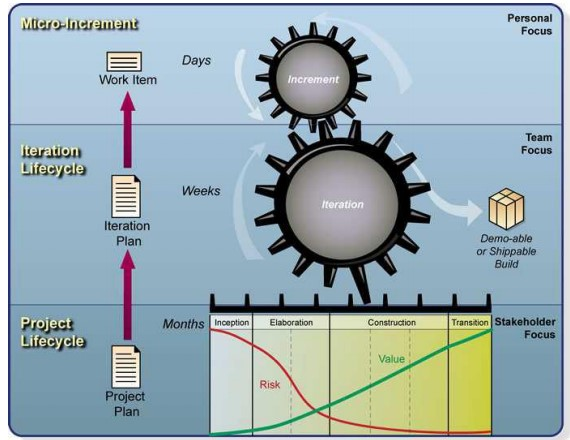
\includegraphics[width=0.5\textwidth]{organizacaoTrabOpenUP.JPG} % leia abaixo
\caption{Organização do trabalho e foco do conteúdo no \textit{OpenUP} \cite{openUP:agil}}
\end{figure}

Papéis definidos pelo \textit{OpenUP}:

\begin{itemize}
\item \textbf{\textit{Stakeholder:}} Representa o interesse do grupo cujas necessidades devem ser satisfeitas
pelo projeto. Esse é um papel que pode ser executado por qualquer um que é (ou
potencialmente será) afetado materialmente pelo resultado do projeto,
\item \textbf{Analista:}  representa o cliente e o usuário final no que diz respeito a obter a entrada
dos \textit{stakeholders} para entender o problema a ser resolvido e pela captura e
configuração das prioridades para os requisitos.
\item \textbf{Arquiteto:} É responsável por projetar a arquitetura do software, que inclui tomar as
decisões técnicas que definem todo o design e implementação do projeto.
\item \textbf{Desenvolvedor:} é responsável por desenvolver uma parte do sistema, inclusive projetá-
lo de acordo com a arquitetura, e então implementá-lo, executar testes unitários e
integrar os componentes que fazem parte da solução.
\item \textbf{Testador:} É responsável pelas principais atividades de testes, como identificar, definir,
implementar e conduzir os testes necessários, bem como registrar as saídas dos testes
e analisar os resultados.
\item \textbf{Gerente de projetos:} lidera o planejamento do projeto em colaboração com os
\textit{stakeholders} e o time, coordenando interações com os \textit{stakeholders}, e mantendo o
time do projeto focado em atingir os objetivos do projeto.
\item \textbf{Qualquer papel:} representa alguém no time que pode realizar tarefas gerais.
\end{itemize}

\subsubsection{Implantação e gerenciamento de processos com AADSP}
O LABRASOFT, Grupo de Pesquisa Laboratório de Desenvolvimento de \textit{Software}, propõe uma abordagem adaptativa para implantação do processo de \textit{software} em empresas soteropolitanas de micro e pequeno porte. A \textit{Adaptive Approach for Deployment of Software Process} tem como alicerce práticas inovadoras em conformidade com o modelo MPS-BR, desenvolvido no Brasil pela SOFTEX (SOFTEX, 2012), práticas de métodos ágeis e o guia de conhecimento PMBOK da PMI (\textit{Project Management Institute}) para gerenciamento de projetos, sendo adaptativa aos diversos perfis das micro e pequenas empresas - MPEs \cite{aadsp:hibirdo}. 

\subsubsection*{Valoração dos artefatos}
A AADSP qualifica os artefatos de acordo com seu grau de importância, desse modo esta abordagem busca a implementação de forma adaptativa nas MPEs. Os três graus de importância são:

\begin{itemize}
\item \textbf{ESSENCIAL:} Artefatos base para implementação do modelo AADSP, de modo que sua continuidade deverá ser garantida objetivando os resultados propostos pela abordagem\cite{aadsp:hibirdo}.
\item \textbf{IMPORTANTE:} Artefatos que são consideráveis, todavia não são obrigatórios, assim sua implementação resultará em resultados adicionais ao modelo\cite{aadsp:hibirdo}.
\item \textbf{DESEJÁVEL:} Artefatos pouco consideráveis, estes não implicam necessariamente na melhoria do processo ou em resultados satisfatórios\cite{aadsp:hibirdo}.
\end{itemize}

\begin{figure}[h]
\centering % para centralizarmos a figura
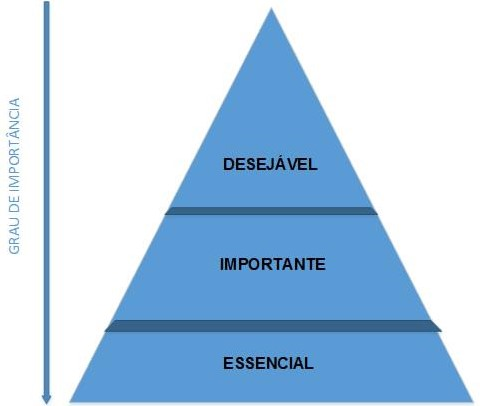
\includegraphics[width=0.5\textwidth]{AADSP_Piramidade_de_importancia_dos_artefatos.jpg} % leia abaixo
\caption{Pirâmide da importância dos artefatos do projeto de \textit{software} na abordagem AADSP  \cite{aadsp:hibirdo}}
\end{figure}

\subsubsection*{Definição da valoração dos artefatos}
A abordagem AADSP  exige que todos os artefatos que afetam o trabalho estejam integrados. Esta abordagem explicita a dependência entre eles e a define no chamado fluxo de trabalho\cite{aadsp:hibirdo}.

\subsubsection*{Confidencialidade e acesso aos artefatos do projeto de software}
A confidencialidade de acesso aos artefatos, mesmo quando não declarada pelo cliente, são contempladas pela abordagem. É recomendável, portanto, explicitar a existência, ou não, de dados confidenciais e acessos a estes\cite{aadsp:hibirdo}.

\subsubsection*{Analise da viabilidade do projeto e comprometimento da equipe executora}
A abordagem AADSP exige que o gerente de projeto reavalie a viabilidade do projeto periodicamente, ou caso de mudança ou acréscimo no escopo de requisito ou de qualquer dos recursos existentes do projeto\cite{aadsp:hibirdo}.

\subsubsection*{Monitoramento contínuo dos artefatos e definição de marcos de trabalho do projeto de software}
Os marcos de trabalho não dependem das cerimônias de revisão realizada dentro do projeto de \textit{software}.  A abordagem AADSP exige o acompanhamento contínuo do projeto comparando o planejado com o realizado. Além disso, deve ser definido no projeto os pontos dentro da escala de importância dos artefatos do projeto. 

\begin{table*}[h]
\scriptsize
\caption{Análise do produto de trabalho MR-MPS e a abordagem híbrida \textit{OpenUP} \cite{Arimoto:melhoria}} 
\centering
\begin{tabular}{|p{20mm}|p{10mm}|p{60mm}|p{60mm}|}
\hline
\textbf{Gerenciamento} & \textbf{Seção} & \textbf{MR-MPS} & \textbf{Abordagem Híbrida} \\
\hline
\multirow{5}{*}{Requisitos} & 1 & Critérios de avaliação e aceitação de requisitos / exigências de documentos & 
Discussões face-a-face / sistema de pesos para os requisitos / modelo de caso de uso / \textit{check List} de tarefas\\
& 2 & Aprovação de requisitos / avaliação de impacto & Discussões face-a-face / \textit{check list} de tarefas \\
& 3 & Sistema de rastreamento de requisitos e produtos de trabalho / matriz de rastreabilidade de requisitos e produtos de trabalho
& -- \\
& 4 & Resultados de revisões / documentação das inconsistências / Ações corretivas & Registros no plano de interação / lista dos itens de trabalho \\
& 5 & status dos requisitos / Repositório dos requisitos / histórico de solicitações e decisões & Lista de itens de trabalho \\
\hline
\multirow{14}{*}{Projetos} & 1 & Estrutura Analítica do projeto (EAP) ou documento de visão & Documento de visão \\
& 2 & Estimativa de tamanho &  estimativa ágil de tamanho ( medido tipicamente usando uma unidade neutra tal como pontos ) \\
& 3 & Fases e ciclos do projeto & Fases do ciclo de vida do projeto (especificada no plano de projeto) \\
& 4 & Estimativas esforço do projeto / as estimativas de custos do projeto & Normalmente usando as unidades de dias efetivos ou horas Reais / cálculo do custo aproximado por pessoa pelo tamanho de uma iteração \\
& 5 & Cronograma e orçamento do projeto & Cronograma do projeto e orçamento (especificada no plano de iteração e do plano do projeto) \\
& 6 & Plano de gestão de risco & Os riscos são identificados / avaliação do impacto e da probabilidade de ocorrência (especificado no plano de projeto ou plano de iteração) / lista de riscos \\
& 7,8 & Plano de gestão de recursos & Plano do projeto / plano de iterações / lista dos itens de trabalho \\
& 9 & plano de gestão de dados & plano de iteração \\
& 10 & Plano geral do projeto & Plano do projeto \\
& 11,12 & Estudo de viabilidade / revisão e compromisso com o plano de projeto & Plano do projeto / discussões face-a-face \\
& 13 & Avaliação do progresso do projeto / status do projeto & Plano de iteração / relatórios (\textit{iteration burndown
e project burndown})\\
& 14 & Plano de gestão de comunicação & plano de iterações / plano do projeto \\
& 15 & Revisão do resultados documentados no projeto & Plano de documentação das iterações \\
& 16,17 & Registro de problemas e monitoramento da ações corretivas / ações corretivas plano & Revisão dos itens de trabalho / plano de iteração \\

\hline
\end{tabular}
\end{table*}

\subsubsection*{Gerências}

\begin{itemize}
\item Gerência de projetos;
\item Gerência de requisitos e modelagem;
\item Gerência de configuração e mudanças;
\item Gerência de colaboradores;
\item Gerência de testes.
\end{itemize}

Este trabalho será focado na gerência de projetos. Deste modo, devemos contemplar os seguintes artefatos definidos para esta gerência:

\begin{itemize}
\item Termo de abertura do  projeto de \textit{software} – TAP (essencial);
\item Estrutura analítica do projeto de \textit{software} – EAP (essencial);
\item Documento de estimativa de escopo (essencial);
\item Definição das funções da equipe executora do projeto (essencial);
\item Cronograma de execução do projeto de \textit{software} (essencial);
\item Orçamento do projeto (essencial);
\item Recursos especiais (importante);
\item Plano organizacional de dados ou plano de gerenciamento de dados  (importante);
\item Plano de riscos do projeto (desejável).
\end{itemize}

\begin{table*}[h]
\scriptsize
\caption{Análise comparativa entre os trabalhos relacionados} 
\centering
\begin{tabular}{|p{60mm}|p{15mm}|p{15mm}|p{15mm}|p{15mm}|p{15mm}|}
\hline
 \textbf{Característica} & \textbf{Bitrix24} & \textbf{Jira} & \textbf{Wrike} & \textbf{T-AADSP} & \textbf{Redmine} \\
\hline
Versão \textit{web} & x & x  & x  & x  & x\\
Sistema de autenticação & x & x  & x  & x & x\\
Definição de cronograma do projeto & x & x  & x  & x  & \\
Definição de termo de abertura de projeto (TAP) &  &   &  & x  & \\
Definição de equipe executora do projeto & x & x  & x  & x  &\\
Controle de reuniões do projeto  & x & x  & x  & x  & x\\
Definição da estrutura analítica do projeto (EAP) &  &   &  & x & \\
Definição da estrutura analítica do projeto (WBS) &  &   &  &  & x \\
Controle dos recursos especiais do projeto &  &   &  & x  &\\
Controle de acesso aos conteúdos da plataforma & x & x  & x  & x & x\\
Mensuração de projeto de software por análise de ponto de função  &  &   &  & x & \\
Controle do projeto por meio do \textit{Smart Gantt chart helps plan} project   &  &   &  &  & x \\
Acompanhamento da execução das etapas do projeto x & x & x & x & x & x\\
\hline
\end{tabular}
\end{table*}

\subsubsection*{Fluxo de trabalho}
Para o AADSP o fluxo de trabalho é uma trilha que conecta os artefatos. Esta trilha pode ser caracterizada por uma sequência contínua de fatos ou operações que apresentam certa unidade. Dessa forma, um artefato é o resultado de um fluxo de trabalho executado \cite{aadsp:hibirdo}.

\begin{figure}[h]
\centering % para centralizarmos a figura
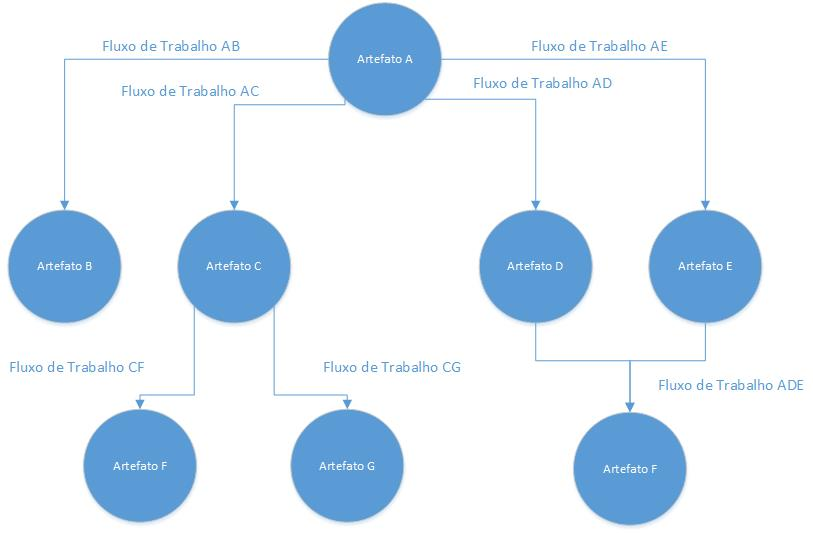
\includegraphics[width=0.5\textwidth]{AADSP_fluxo_de_trabalho.jpg} % leia abaixo
\caption{Fluxo de trabalho em um projeto de \textit{software} na abordagem AADSP  \cite{aadsp:hibirdo}}
\end{figure}

A abordagem AADSP é voltada a artefatos, e deste modo, os processos são comprovados a partir da existência dos mesmos em um projeto de \textit{software} que implemente esta metodologia. A segmentação das gerências determinam quais artefatos estão sob a responsabilidade da mesma e o fato desta valorar seus artefatos promovem adaptabilidade ao projeto, que deste modo, não dependerá do tamanho de uma equipe para implantação ou tecnologias adotadas, permitindo maior fluidez no gerenciamento do projeto de software.

\subsection{Melhoria do processo de software x métodos ágeis}
Nesta seção será discutido as abordagens para melhoria do processo de desenvolvimento de \textit{software} em comparativo ao desenvolvimento ágil de \textit{software}. Será considerado para este comparativo a abordagem do MPS.BR desenvolvido pela Associação para Promoção da Excelência do \textit{Software} Brasileiro (SOFTEX) e os modelos de desenvolvimento de \textit{software} baseado no Manifesto Ágil para Desenvolvimento de \textit{Software}. Um aspecto que diferencia os métodos ágeis de um modelo de referência, tais como MR-MPS e
outras abordagens convencionais é a granularidade que algumas atividades são realizadas. Portanto, algumas atividades podem executar a mesma função nos dois modelos, mas com um nível diferente de profundidade. Assim, um elemento de fundamental
característica técnica para avaliar a percentagem de adesão entre os métodos ágeis e os modelos de maturidade é a realização de uma análise detalhada, considerando as características particulares de cada um deles \cite{Arimoto:melhoria}.  

Esta análise é um comparativo do modelo de adesão ao MR-MPS-SW:2012 Nível G, Arimoto \cite{Arimoto:melhoria} realizou o comparativo entre os modelos e tabulou os seguintes resultados conforme apresentados na tabela 2.

Arimoto \cite{Arimoto:melhoria} incluiu em seu quadro comparativo o \textit{OpenUP}, que para este trabalho será qualificado enquanto abordagem híbrida para melhoria de processo de \textit{software}, mediante ser fundamentada no \textit{Rational Unified Process} - RUP (ou Processo Unificado da Rational).

Neste trabalho foi realizado um comparativo entre abordagem MR-MPS.SW e a abordagem híbrida AADSP, além de demonstrar em quais requisitos da ferramenta T-AADSP foi contemplado este artefato, conforme demonstrado na tabela 1.

Castro \cite{Castro:melhoria} afirma que não é fácil definir o conjunto de práticas que deveriam ser utilizadas numa organização, desde a sua implantação, passando pela sua manutenção e evolução \cite{Castro:melhoria}. A prática pode ser a mesma, mas a forma da implementação pode ser diferente de organização para organização. Desse modo, a abordagem deve promover certa “adaptabilidade” durante seu processo de implantação. 

Realizando um comparativo do MR-MPS.SW:2012 nível G e abordagem a AADSP, podemos observar que esta última, por ser uma abordagem híbrida, elenca práticas ágeis, ao mesmo tempo que considera fundamental a existência e manutenibilidade dos artefatos documentais do projeto. Já o MR-MPS.SW:2012 nível G não aborda as práticas ágeis, apenas denifindo os artefatos documentais esperados ao projeto. Castro \cite{Castro:melhoria} explicita que apesar da especificação de cada prática apresentar uma simplicidade na sua implementação, não se pode assumir que sejam simples de serem aplicadas em um projeto. Além do fato que é necessária a integração de práticas de outros métodos \cite{Castro:melhoria}. Na prática, em ambientes ágeis, essa integração a outras práticas pode surgir das retrospectivas e reuniões para análise e melhoria contínua do trabalho, porém uma única abordagem ágil também não seria capaz de contemplar todos resultados esperados pelo MR-MPS.SW \cite{Castro:melhoria}. A abordagem AADSP demonstrou contemplar os resultados esperados pela implantação MR-MPS.SW nível G como demonstrado na tabela 2.


\section{Trabalhos relacionados}
Nesta seção foram selecionadas três ferramentas, onde foi analisada as suas funcionalidades que estão disponibilizadas aos usuários. São descritas, a seguir, as principais características das ferramentas analisadas:

\begin{itemize}
\item \textbf{Bitrix24:} É uma plataforma completa de colaboração social, comunicação e ferramentas de gestão. Esta ferramenta trabalha integrada as redes sociais corporativas, disseminando postagens e comunicados. Esta ferramenta trabalha com gerenciamento de projetos / grupos de trabalho, tarefas e subtarefas, modelos de tarefa, tarefas recorrentes, gerenciamento de registros (Listas), diagrama de Gantt, gerenciamento de tempo \cite{bitrix24:ferramenta}.
\item \textbf{Jira:}  Permite a gestão, criação e delegação de projetos e tarefas, com fluxos de processos personalizados para o acompanhamento dos projetos, controle de acesso e segurança customizado, acesso via web com suporte aos principais \textit{browsers} do mercado, notificações / alertas por \textit{email},  centenas de \textit{plug-ins} gratuitos. É uma ferramenta robusta para gestão de projetos e tarefas, bem como para acompanhamento e reporte de defeitos (\textit{bugs}) em projetos de qualquer natureza \cite{jira:ferramenta}.
\item \textbf{Wrike:} É uma ferramenta interativa para colaboração, planejamento de projetos, otimização de carga de trabalho e acompanhamento do andamento. Ajudam a equipe a produzir mais e com maior velocidade, independente de onde se encontrem. Além disso, as notificações em tempo real apresentam todas as atualizações diárias das atividades do projeto, eliminando a necessidade de reuniões extras e \textit{e-mails}. Os painéis personalizáveis ajudam a monitorar projetos específicos, etapas importantes, trabalhos delegados, entre outros.  
\item \textbf{Redmine:} É uma plataforma para gerenciamento de projetos. Esta ferramenta permite gerenciar projetos complexos de forma rápida através de diagramas e componentes de fácil manipulação como o diagrama \textit{Smart Gantt chart}. A ferramenta também promove maior velocidade no controle e comunicação de tarefas, além de permitir o gerenciamento de projetos simultâneos e dos repositórios de integração do projeto.
\end{itemize}

\subsection{Comparativo entre ferramentas}
 A Tabela 2 exibe uma análise comparativa entre as ferramentas estudadas.

Conforme explanado na tabela 2, existem diversas soluções para gerenciamento de projetos. Este trabalho, assim como a abordagem AADSP, propõe um modelo alternativo para o gerenciamento de projetos de \textit{software}, justificando então a sua escolha. Destacam-se na ferramenta os recursos como mensuração do tamanho de \textit{software}, através da métrica de analise por ponto de função, controle do escopo do projeto através de diagrama da estrutura analítica do projeto e gerenciamento do termo de abertura de projetos. 

\section{A ferramenta T-AADSP}
O T-AADSP é uma ferramenta para a implantação e o gerenciamento de processos em projetos de \textit{software}. Para construção deste sistema foi necessário seguir as etapas inerentes ao projeto de desenvolvimento de sistemas (Levantamento de Requisitos, Análise, Projeto, implementação e Testes).
Serão apresentados, a seguir, as etapas realizadas para o desenvolvimento da ferramenta T-AADSP.

\subsection{Requisitos do sistema}
Os requisitos funcionais do sistema serão apresentados a seguir, estes foram separados em: Requisitos Funcionais e Não Funcionais.

\subsection{Requisitos funcionais}
As principais funcionalidades da ferramenta serão descritas
nas subsecções seguintes, vale ressaltar, que devido ao porte desta ferramenta só elencaremos alguns dos requisitos desenvolvidos:

\subsubsection{Autenticação}
Para o usuário ter acesso de login, este deve ter sido cadastrado previamente no sistema. Em caso de uma nova instalação do sistema, por definição padrão, o banco de dados virá configurado com um usuário administrador com acesso a todas as páginas do sistema. Para acessar com este usuário deverá ser informado os seguintes dados de acesso: login = adm e senha = aadsp (figura 5). Caso seja informado dados incorretos, a ferramenta informará a mensagem de alerta "Não foi possível realizar a autenticação do usuário!" (figura 6), caso somente a senha esteja incorreta o sistema irá informar "Senha incorreta!" (figura 7)

\subsubsection{Solicitar nova senha}
Este requisito possibilitará ao usuário solicitar uma nova senha, via e-mail, para isso o usuário deverá fornecer o e-mail dele e o sistema verificará a existência do e-mail informado pelo usuário e enviará uma nova senha definida automaticamente pelo sistema (figura 8). Caso o sistema envie a nova senha ao e-mail, este exibirá a mensagem "senha enviada com sucesso" (figura 9), porém se este não conseguir enviar a nova senha, via e-mail, o sistema exibirá a seguinte mensagem "Não foi possível realizar o envio de uma nova senha para este e-mail, por favor, tente novamente mais tarde!" (figura 10)

\subsubsection{Cadastro de usuário}
Para o usuário ter acesso ao sistema deverá ser realizado um cadastro por um usuário administrador. Deve ser fornecido os seguintes dados: nome completo, data de nascimento, RG, CPF, e-mail, login, senha, função que irá desempenhar no sistema, e ao final clicar, no botão cadastrar conforme exibido na figura 11.

\subsubsection{Consulta de pessoal}
O usuário autenticado, que possua permissões de acesso a este requisito, poderá consultar o pessoal cadastrado no sistema. Nesta tela é possível filtrar informações referentes aos usuários cadastrados como: nome, e-mail, login de acesso.   

\subsubsection{Definir permissão de acesso por função do usuário}
O usuário poderá definir acesso as funcionalidades do sistema de acordo com a função do usuário. Desse modo deve ser selecionada a função do usuário e selecionada a tela a qual este terá permissão, as ações nas telas estão segmentadas de acordo com sua característica exemplo: consulta e impressão, cadastro, edição e exclusão. 

\subsubsection{Cadastro de paginas}
O usuário poderá definir quais páginas será passíveis de acesso no sistema, estas páginas permitirão controlar o acesso do usuário, por função, no sistema.

\subsubsection{Alterar senha}
O usuário poderá modificar sua senha por meio deste requisito. O Sistema solicitará que o usuário forneça um nova senha e, em seguida, confirme esta senha. Será informado o grau de dificuldade da senha informada.

\subsubsection{Consulta dos termos de abertura de projeto}
O usuário poderá consultar todos os termos de abertura de projeto de software. O termo de abertura de projeto de \textit{software} é o primeiro documento a ser gerenciado na ferramenta. No termo de abertura irá conter as definições iniciais de um projeto de desenvolvimento de software, além disso, será o primeiro artefato documental a ser homologado junto aos \textit{stakeholders}.

\subsubsection{Consulta dos projetos}
O usuário poderá consultar todos os projetos de desenvolvimento de \textit{software} criados no sistema. Um projeto é oriundo de um termo de abertura de projeto de \textit{software}. Desse modo, todo projeto é fundamentado em um TAP. Cada TAP poderá ter um, e somente um, projeto associado ao mesmo.

\subsubsection{Consulta das atas das reuniões do projeto}
O usuário poderá consultar todas as atas de reuniões cadastradas no sistema. Uma ata de reunião é a formalização de uma cerimônia onde foram definidas ações consagradas e tomadas de decisões no projeto.

\subsubsection{Consulta das estruturas analíticas do projeto}
O usuário poderá cadastrar três tipos distintos de EAP (Pacote, fases, entregas) a um projeto de \textit{software} e visualizar uma EAP na estrutura de um diagrama ou consulta-la por meio de uma lista. 

\subsubsection{Consulta dos documentos de estimativa do escopo do projeto}
O usuário poderá consultar os projetos os quais serão realizados as estimativas de escopo. A estimativa de escopo deverá ser realizada por meio do cálculo do ponto de função do projeto.

\subsubsection{Consulta dos cronogramas de execução do projeto}
O usuário poderá consultar a relação de projetos no sistema, a fim de realizar o cadastro das atividades a compor o mesmos, através de um cronograma de execução dos projetos.

\subsubsection{Consulta dos recursos especiais do projeto}
O usuário poderá consultar os projetos para definição dos recursos especiais por meio do botão detalhar.

\subsubsection{Cadastro do termo de abertura de projeto}
O usuário poderá cadastrar um novo termo de abertura de projeto informando o nome do projeto, justificativa, alinhamento estratégico, orçamento previsto, cronograma inicial, premissas do projeto, restrições do projeto e mensurar os riscos do projeto. 

\subsubsection{Cadastro do projeto}
Um projeto só poderá ser cadastrado mediante existência de um termo de abertura a ser associado ao mesmo. Deve ser informado o valor do projeto e seu cronograma.

\subsubsection{Cadastro das atas das reuniões do projeto}
Poderá ser realizado o cadastro da ata de reunião oriunda de uma cerimônia, que poderá ser consultada posteriormente e homologada junto aos \textit{stakeholders}.

\subsubsection{Cadastro da estrutura analítica do projeto}
Todo projeto poderá possuir três modelos de EAP (Pacote, Entrega e Fase). Deve ser cadastrado o pacote a qual uma atividade será inserida, e desse modo, deve ser cadastrada uma ou mais atividades a compor o pacote cadastrado. É possível visualizar a estrutura do projeto em forma de diagrama. 

\subsubsection{Cadastro dos documentos de estimativa de escopo do projeto}
Para estimar o tamanho do projeto, deverá ser realizado o cálculo dos pontos de função. Para este cálculo, poderá ser consultado um valor base, como também, as quatorze características gerais dos projetos de software objetivando, os ajuste do pontos de função. Após a inserção dos dados das funções dos tipos de dados e transações, deverá ser informado as características gerais do sistema encontradas. Por fim, o sistema informará automaticamente o valor total dos pontos de funções calculados e o valor ajustado.

\subsubsection{Cadastro do cronograma de execução do projeto}
O usuário poderá definir data para realização de atividades do projeto. Estas datas serão catalogadas em um cronograma de execução de atividades.

\subsubsection{Cadastro dos recursos especiais do projeto}
O usuário poderá cadastrar os recursos especiais do projeto. Para cadastrar um novo recurso deverá ser informado o nome do recurso e o valor do mesmo.

\subsubsection{Detalhamento de informações do projeto}
Neste requisito será possível informar demais informações ao projeto, como equipe executora, visualizar as funções definidas ao projeto por meio do TAP. Também será possível visualizar estas informações por meio de visualizações de dados. Através deste requisito, o usuário poderá alterar as informações do projeto. 

\subsubsection{Detalhamento de atas das reuniões do projeto}
Neste requisito será possível detalhar as informações de uma determinada ata de reunião, podendo também ser alterado os dados existentes como: título, data realização, organizador, além da pauta e assuntos tratados.

\subsubsection{Detalhamento da estrutura analítica do projeto}
Através deste requisito será possível detalhar informações ao mesmo tempo que editar/excluir informações já inseridas.

\section{Fluxo básico da ferramenta T-AADSP}
Nesta seção serão apresentados os referidos casos de uso dos requisitos anteriormente mencionados, devido ao tamanho da ferramenta serão elencados apenas alguns dos casos de uso que fazem parte da ferramenta.

\begin{figure*}[h]
\centering % para centralizarmos a figura
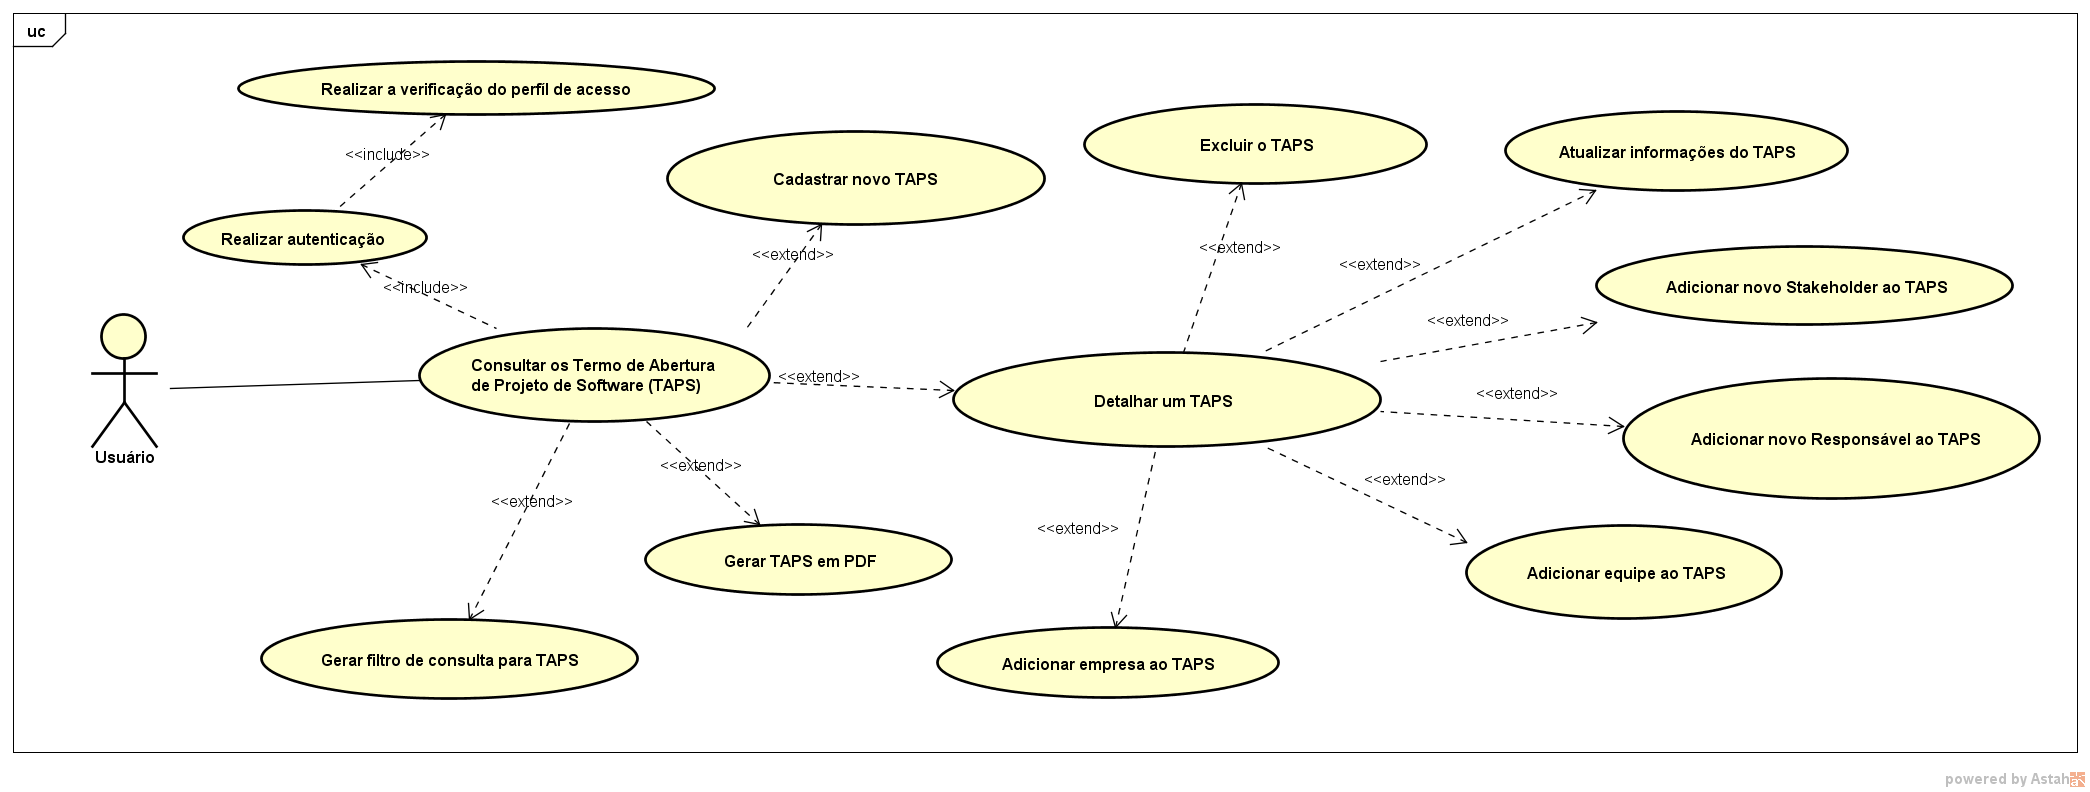
\includegraphics[width=1\textwidth]{TAP.png} % leia abaixo
\caption{PROJETO - Termo de abertura do projeto de  \textit{software}}
\end{figure*}

\begin{figure*}[h]
\centering % para centralizarmos a figura
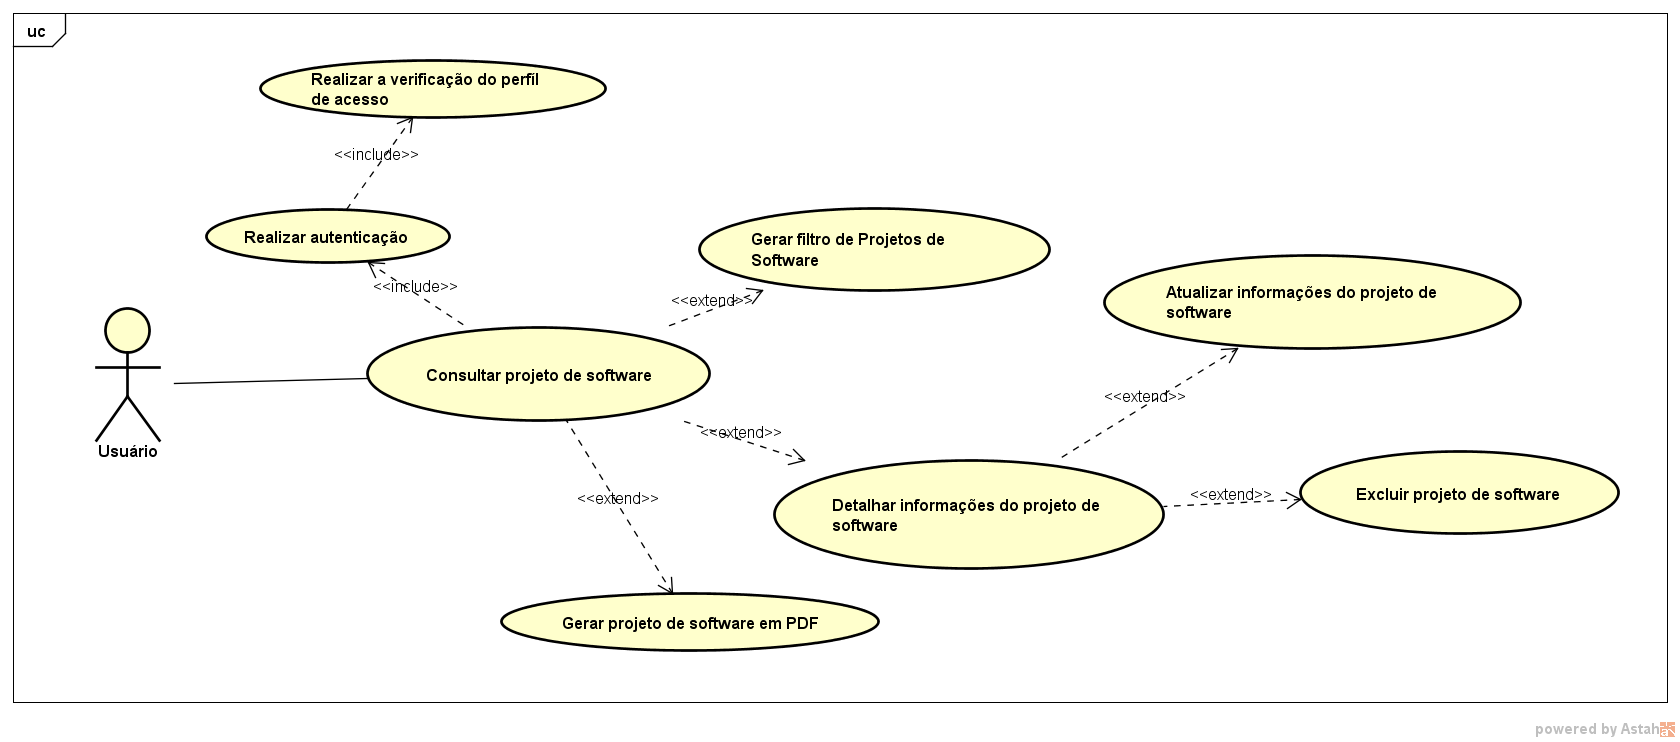
\includegraphics[width=1\textwidth]{Consulta_de_Projeto.png} % leia abaixo
\caption{PROJETO - Projetos de  \textit{software}}
\end{figure*}

\begin{figure*}[h]
\centering % para centralizarmos a figura
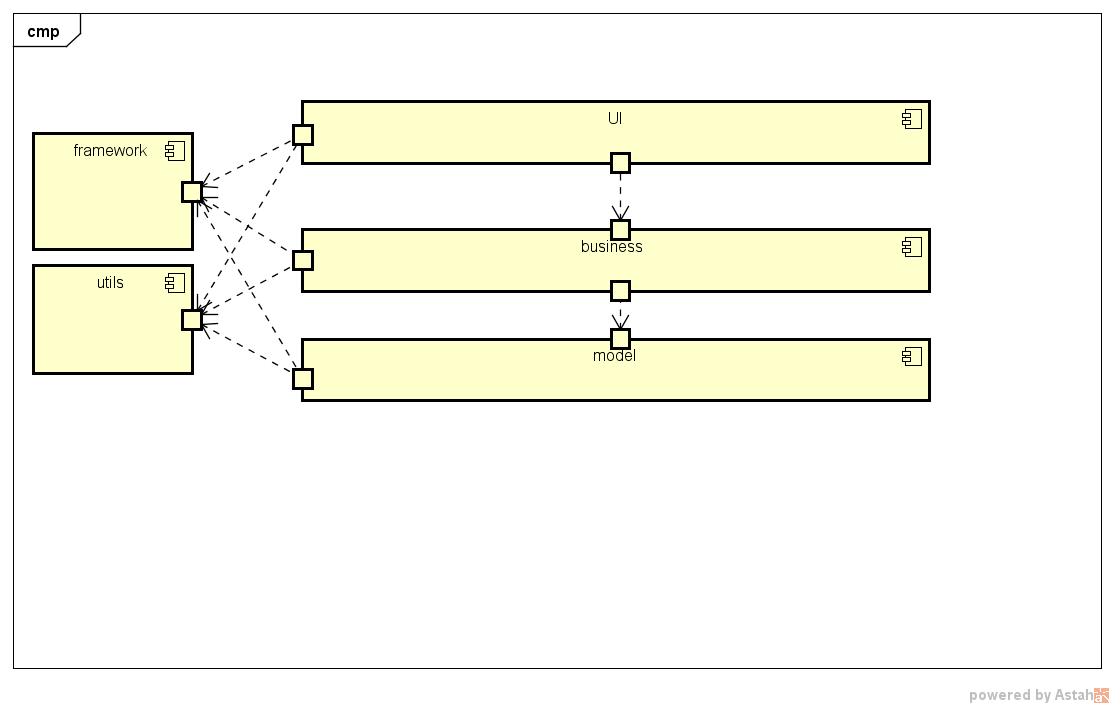
\includegraphics[width=1\textwidth]{ArquiteturaDoProjeto.png} % leia abaixo
\caption{Diagrama da arquitetura do \textit{software}}
\end{figure*}

\section{Desenvolvimento da ferramenta T-AADSP}
\subsection{Tecnologias utilizadas}
Este projeto foi todo desenvolvido utilizando as seguintes tecnologias:

\begin{itemize}
\item \textbf{Servidor para o web:} \textit{GlassFish} 4.1.1. 
\item \textbf{\textit{Apache Maven Project}:} \textit{Apache Maven} é uma ferramenta de gerenciamento de projetos de \textit{software} e compreensão. Baseado no conceito de um modelo de objeto de projeto (POM), \textit{Maven} pode gerenciar construção de um projeto, elaboração de relatórios e documentação de uma peça central de informações.
\item \textbf{JSF 2.2:}\textit{Java Server Faces} (JSF) é uma especificação Java para a construção de interfaces de usuário baseadas em componentes para aplicações \textit{web}.
\item \textbf{\textit{Primefaces} 5.3:} \textit{PrimeFaces} é um \textit{open source User Interface} biblioteca (UI) componentes para \textit{JavaServer Faces} (JSF) aplicações baseadas, criados por \textit{PrimeTek}.  
\item \textbf{\textit{Bootstrap} 2.3.2:} \textit{Bootstrap} é uma estrutura de \textit{front-end} elegante, intuitiva e poderosa para o desenvolvimento \textit{web} mais rápida e fácil, criado por Mark Otto e Jacob Thornton , e mantida pela equipe principal com o apoio maciço e envolvimento da comunidade. 
\item \textbf{\textit{Hibernate} 4.3.6:} O \textit{Hibernate} é um \textit{framework} para o mapeamento objeto-relacional escrito na linguagem Java. 
\item \textbf{SGBD (Sistema de Gerenciamento de Banco de Dados):}\textit{SQLServer} 2008. 
\end{itemize}


\section{Projeto em estudo}
A ferramenta T-AADSP foi implantada na empresa Computação Brasil, empresa que atua no segmento do desenvolvimento de \textit{softwares} corporativos desde 2008. Participaram desta etapa do projeto três pessoas, todos da área da computação. O período de utilização da ferramenta foi de 01/06/2016 à 20/07/2016. 

Os participantes testaram as funcionalidades contidas na ferramenta T-AADSP, utilizando para isto projetos reais. Vale ressaltar, que esta empresa já utilizava a abordagem AADSP para melhoria do processo de software, sem o uso da ferramenta. Participaram também dois bolsistas que utilizaram a ferramenta para mensuração de \textit{software} em trabalhos desenvolvidos pelos mesmos na empresa em questão. Os resultados foram coletados e apresentados no apêndice A.

\section{Analise de dados reais}
Foram testados três projetos na ferramenta, todos da área da Computação. Os projetos foram cadastrados e monitoradas pela ferramenta T-AADSP.  

\section{Avaliação da ferramenta}


\section{Conclusão}


%\end{document}  % This is where a 'short' article might terminate

%ACKNOWLEDGMENTS are optional
\bibliographystyle{acm}
\bibliography{sigproc}

\begin{appendices}

\chapter{Tabelas}

\chapter{Requisitos Funcionais}

\chapter{Diagramas UML}

\chapter{Diagrama de Entidade e Relacionamento}

\begin{table*}[h]
\scriptsize
\caption{Análise dos resultados esperados do MR-MPS.SW no nível G e a abordagem híbrida \textit{AADSP} \cite{aadsp:hibirdo}} 
\centering
\begin{tabular}{|p{10mm}|p{60mm}|p{60mm}|p{25mm}|}
\hline
\textbf{GPR} & \textbf{Resultado esperado pelo MR-MPS.SW} & \textbf{Artefato do AADSP que contempla o resultado esperado} & \textbf{Artefato no T-AADSP} \\
\hline
1 & O escopo do trabalho para o projeto é definido & Estrutura analítica do projeto
(Gerência de projetos) & Gerência de projetos \\
2 & As tarefas e os produtos de trabalho do projeto são dimensionados utilizando métodos apropriados & Análise de pontos por função (Gerência de projetos) & Gerência de projetos\\
3 & O modelo e as fases do ciclo de vida do projeto são definidos & Requisitos do projeto são realizados sob ciclos de \textit{Sprint} (Gerência de requisitos) & Não desenvolvido\\
4 &  O esforço e o custo para a execução das tarefas e dos produtos de trabalho são estimados com base em dados históricos ou referências técnicas & Requisitos do projeto são realizados sob ciclos de \textit{Sprint} (Gerência de requisitos), Análise de pontos por função (Gerência de projetos) & Gerência de projetos\\
5 & O orçamento e o cronograma do projeto, incluindo a definição de marcos e pontos de controle, são estabelecidos e mantidos
& Definição e controle do projeto (Gerência de projetos) & Gerência de projetos\\
6 & Os riscos do projeto são identificados e o seu impacto, probabilidade de ocorrência e prioridade de tratamento são
determinados e documentados & Termo de abertura do projeto (Gerência de projetos) & Gerência de projetos\\
7 & Os recursos humanos para o projeto são planejados considerando o perfil e o conhecimento necessários para executá-lo & Definição da função dos colaboradores (Gerência de recursos humanos) & Gerência de projetos\\
8 & Os recursos e o ambiente de trabalho necessários para executar o projeto são planejados & Definição dos recursos necessários ao projeto (Gerência de projetos) & Gerência de projetos\\
9 & Os dados relevantes do projeto são identificados e planejados quanto à forma de coleta, armazenamento e distribuição. Um mecanismo é estabelecido para acessá-los, incluindo, se pertinente, questões de privacidade e segurança & Controle de acesso aos conteúdos (Gerência de projetos) & Gerência de projetos\\
10 & Um plano geral para a execução do projeto é estabelecido com a integração de planos específicos & Cronograma de execução das atividades (Gerência de projetos) & Gerência de projetos\\
11 & A viabilidade de atingir as metas do projeto é explicitamente avaliada considerando restrições e recursos disponíveis. Se necessário, ajustes são realizados & \textit{Check list} do Projeto (Gerência de projetos) & \\
12 & O Plano do projeto é revisado com todos os interessados e o compromisso com ele é obtido e mantido &  \textit{Check list} de revisão do do projeto (Gerência de Projetos)& Gerência de projetos\\
13 & O escopo, as tarefas, as estimativas, o orçamento e o cronograma do projeto são monitorados em relação ao planejado & 
Acompanhamento do Projeto (Gerência de projetos), Acompanhamento do Cronograma do Projeto (Gerência de projetos) & Gerência de projetos\\
14 & Os recursos materiais e humanos bem como os dados relevantes do projeto são monitorados em relação ao planejado & 
Termo de abertura do projeto (Gerência de projetos), Definição e controle do projeto & Gerência de projetos \\
15 & Os riscos são monitorados em relação ao planejado & Termo de abertura do projeto (Gerência de projetos) &  Gerência de projetos\\
16 & O envolvimento das partes interessadas no projeto é planejado, monitorado e mantido & Gerenciamento das atividades do projeto (Gerência de requisitos)  & Não desenvolvido \\
17 & Revisões são realizadas em marcos do projeto e conforme estabelecido no planejamento & Revisões das entregas durante os ciclos da \textit{Sprint} (Gerência de requisitos) & Não Desenvolvido \\
18 & Registros de problemas identificados e o resultado da análise de questões pertinentes, incluindo dependências críticas, são
estabelecidos e tratados com as partes interessadas & Revisões das entregas durante os ciclos da \textit{Sprint} (Gerência de reutilização ) & Não desenvolvido \\
19 & Ações para corrigir desvios em relação ao planejado e para prevenir a repetição dos problemas identificados são estabelecidas, implementadas e acompanhadas até a sua conclusão & Revisões das entregas durante os ciclos da Sprint (Gerência de requisitos) & Não desenvolvido \\

\hline
\end{tabular}
\end{table*}

\begin{figure}[h]
\centering % para centralizarmos a figura
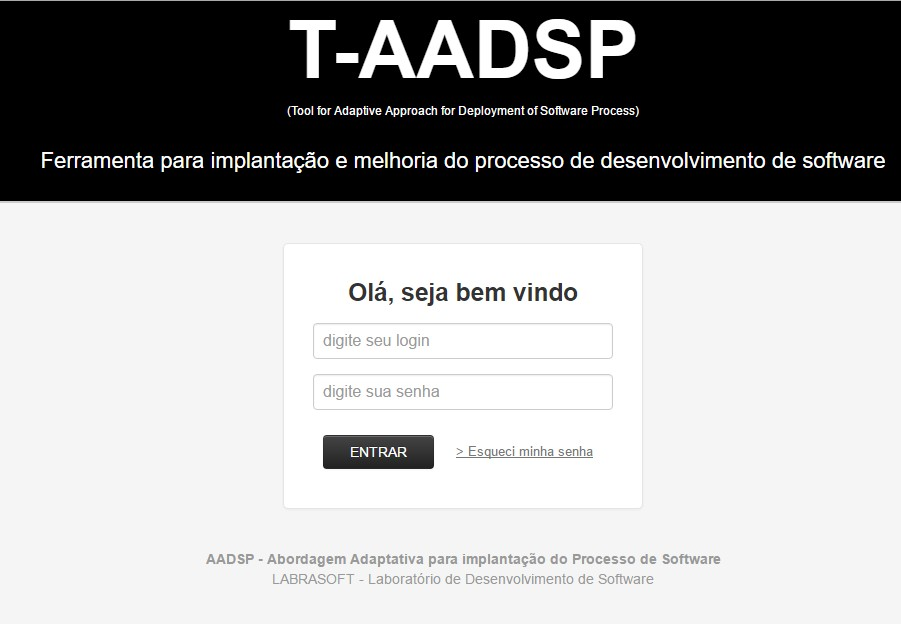
\includegraphics[width=0.5\textwidth]{RF_autenticacao.jpg} % leia abaixo
\caption{Autenticação do sistema T-AADSP}
\end{figure}

\begin{figure}[h]
\centering % para centralizarmos a figura
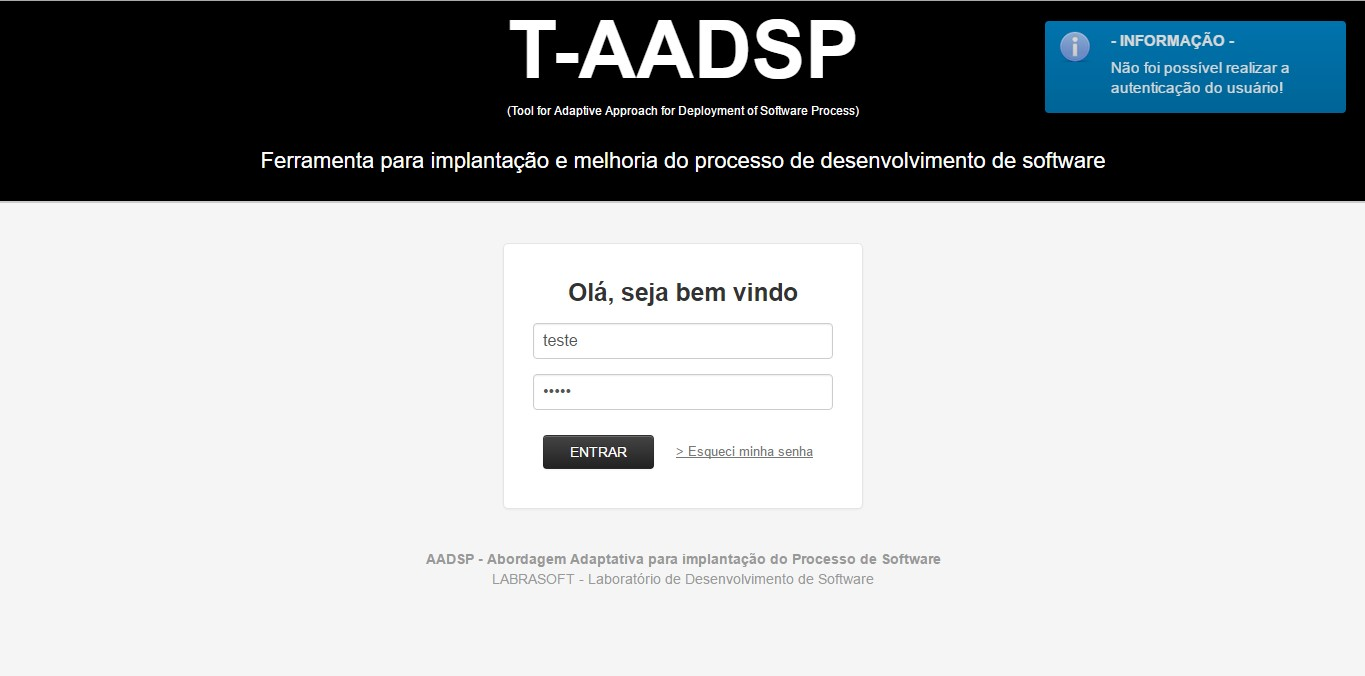
\includegraphics[width=0.5\textwidth]{RF_autenticacao_dados_incorretos.jpg} % leia abaixo
\caption{Mensagem não foi possível realizar a autenticação do usuário! }
\end{figure}

\begin{figure}[h]
\centering % para centralizarmos a figura
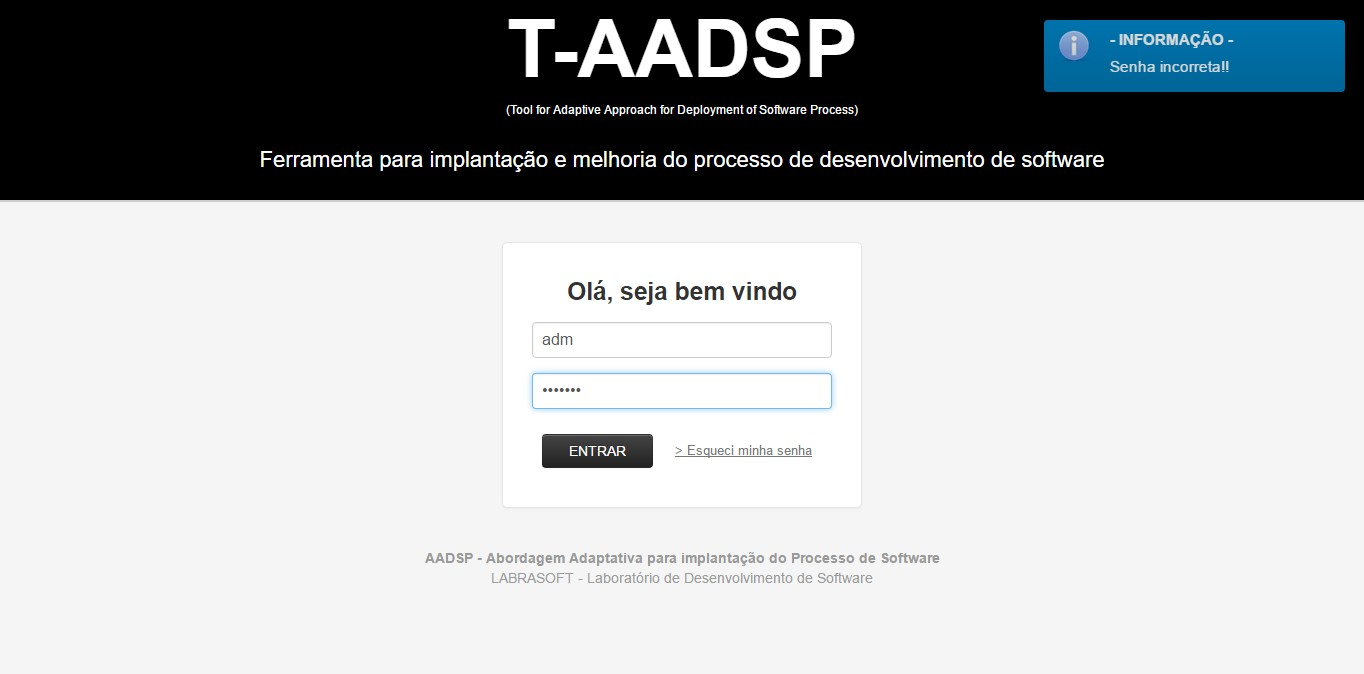
\includegraphics[width=0.5\textwidth]{RF_autenticacao_senha_incorreta.jpg} % leia abaixo
\caption{A senha informada está incorreta! }
\end{figure}

\begin{figure}[h]
\centering % para centralizarmos a figura
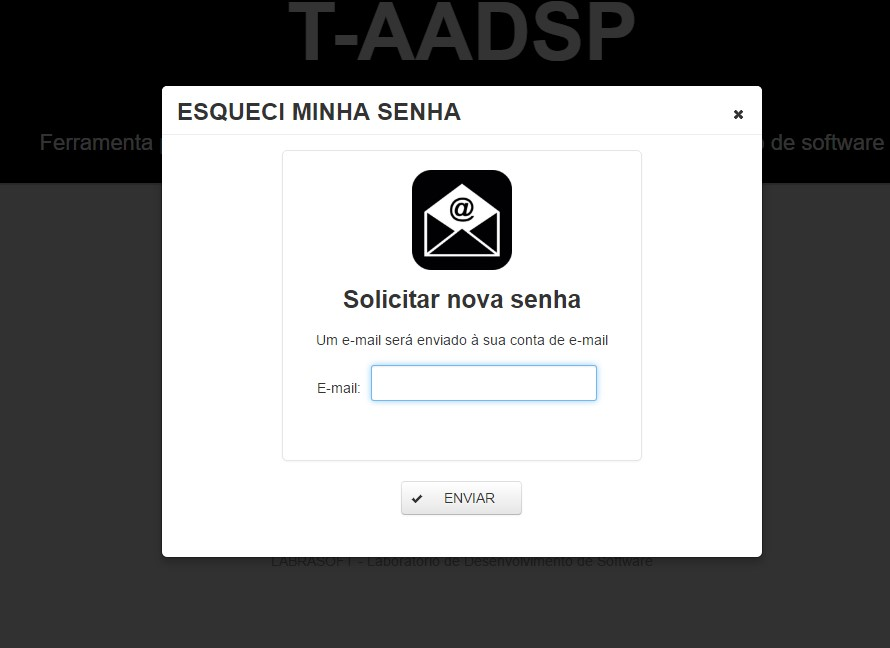
\includegraphics[width=0.5\textwidth]{RF_autenticacao_solicitar_nova_senha.jpg} % leia abaixo
\caption{Solicitação de nova senha via e-mail }
\end{figure}

\begin{figure}[h]
\centering % para centralizarmos a figura
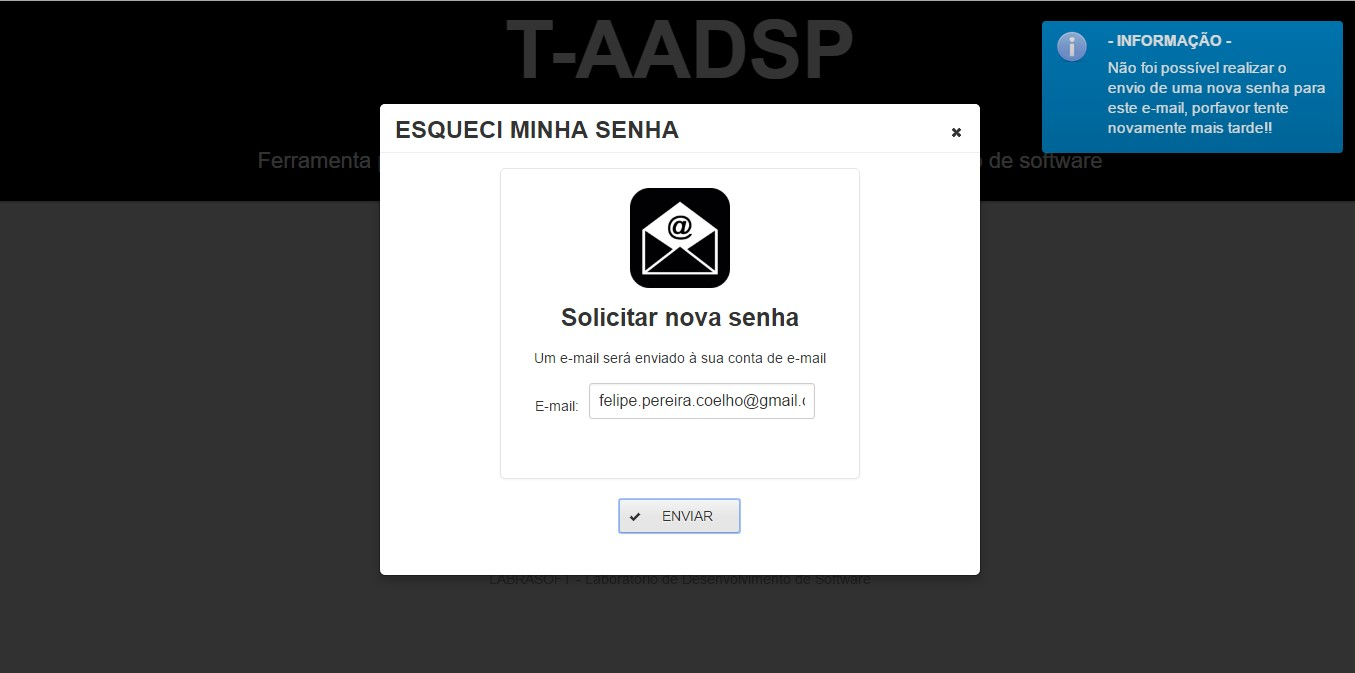
\includegraphics[width=0.5\textwidth]{RF_autenticacao_falha_ao_enviar_senha.jpg} % leia abaixo
\caption{Não foi possível realizar o envio de uma nova senha ao usuário}
\end{figure}

\begin{figure}[h]
\centering % para centralizarmos a figura
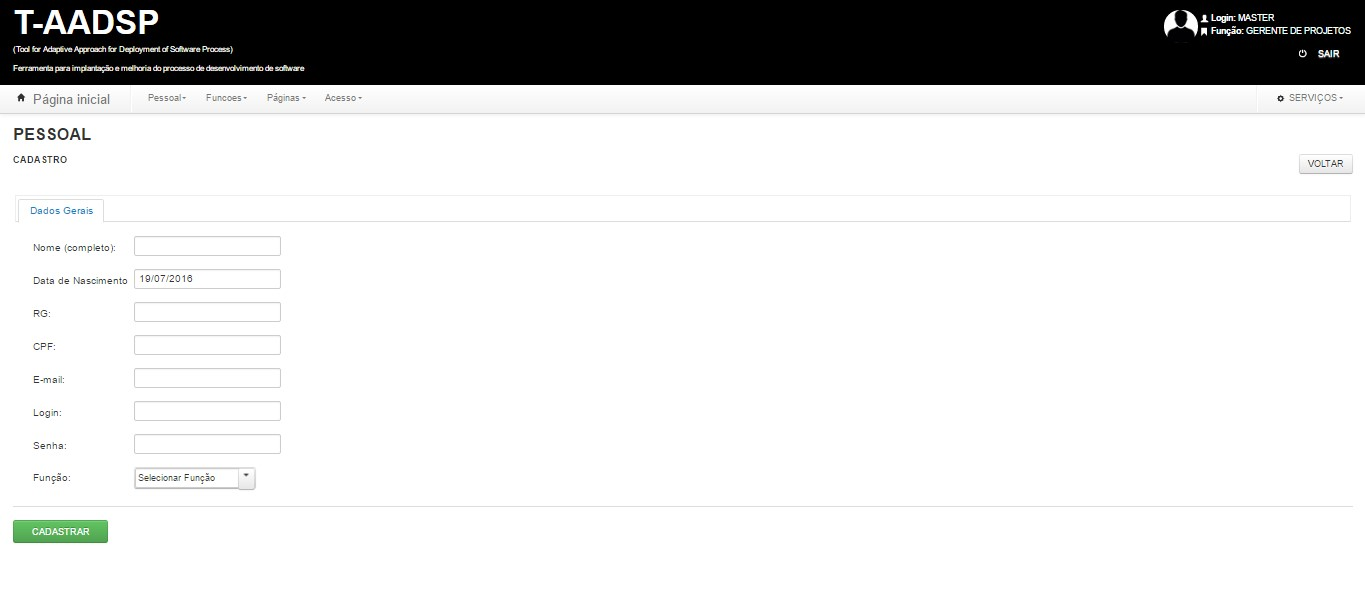
\includegraphics[width=0.5\textwidth]{RF_cadastro_de_usuario.jpg} % leia abaixo
\caption{Cadastrando novos usuários no sistema}
\end{figure}

\begin{figure}[h]
\centering % para centralizarmos a figura
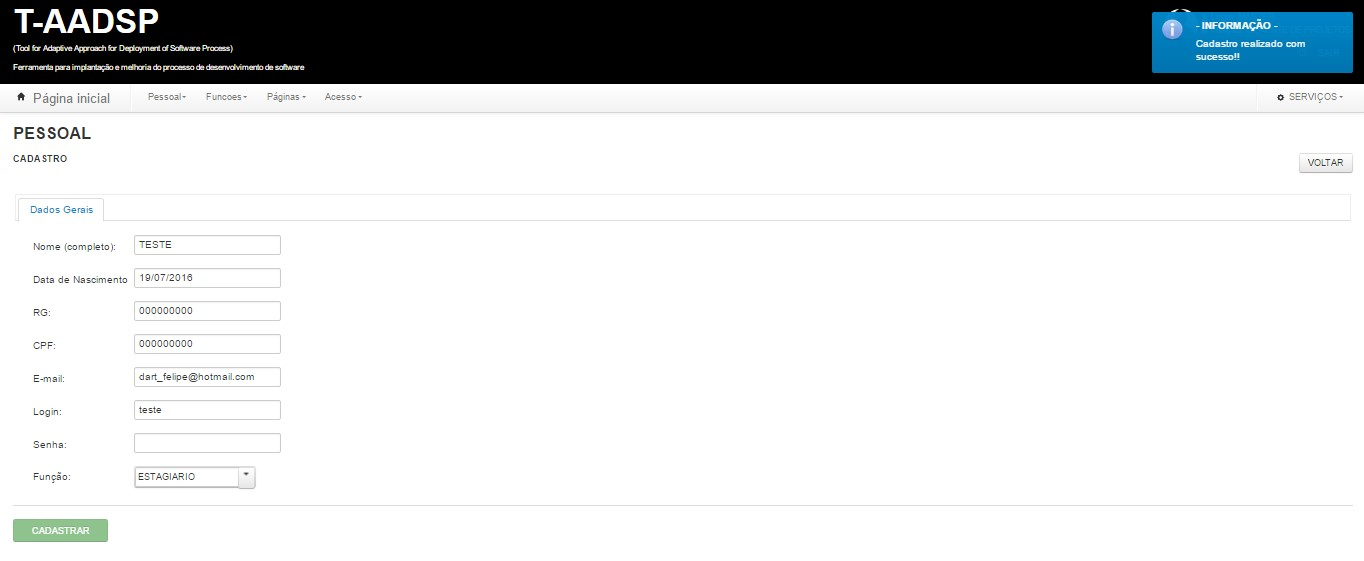
\includegraphics[width=0.5\textwidth]{RF_cadastro_de_usuario_realizado.jpg} % leia abaixo
\caption{Confirmação de novo usuário cadastrado no sistema}
\end{figure}

\begin{figure}[h]
\centering % para centralizarmos a figura
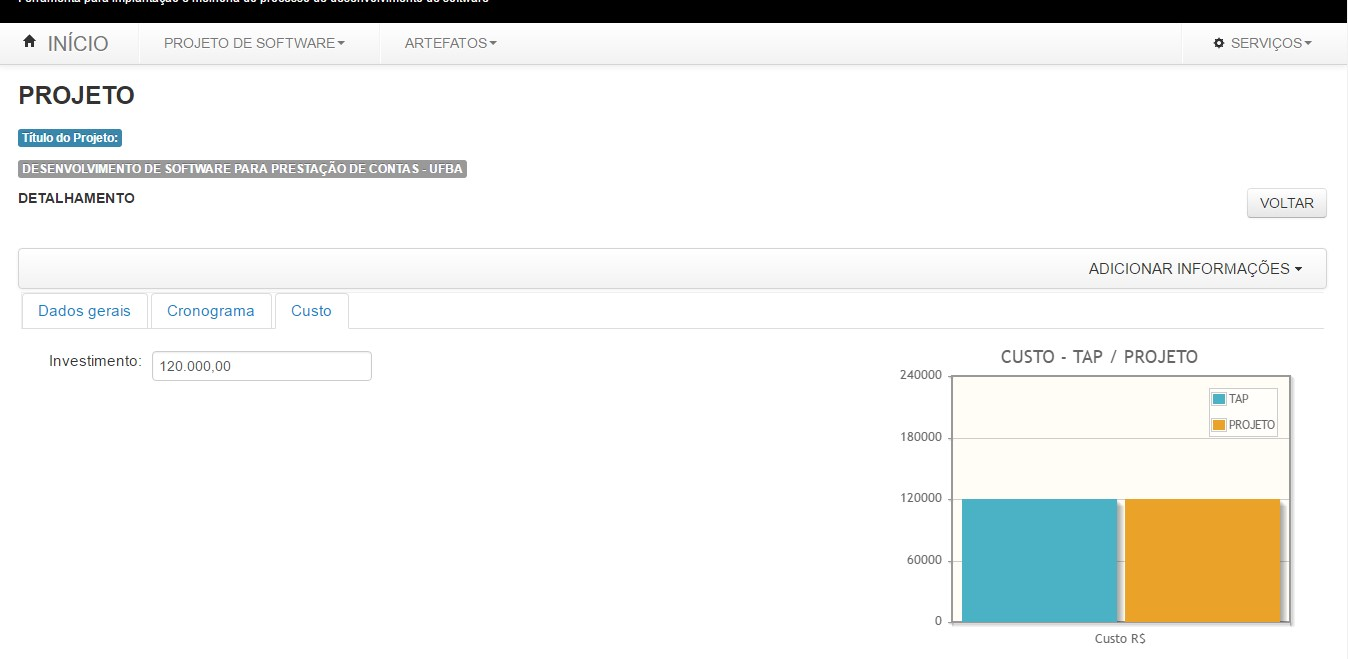
\includegraphics[width=0.5\textwidth]{RF_detalhamento_Projeto.jpg} % leia abaixo
\caption{Detalhes de um projeto cadastrado no sistema em função do seu custo}
\end{figure}

\begin{figure}[h]
\centering % para centralizarmos a figura
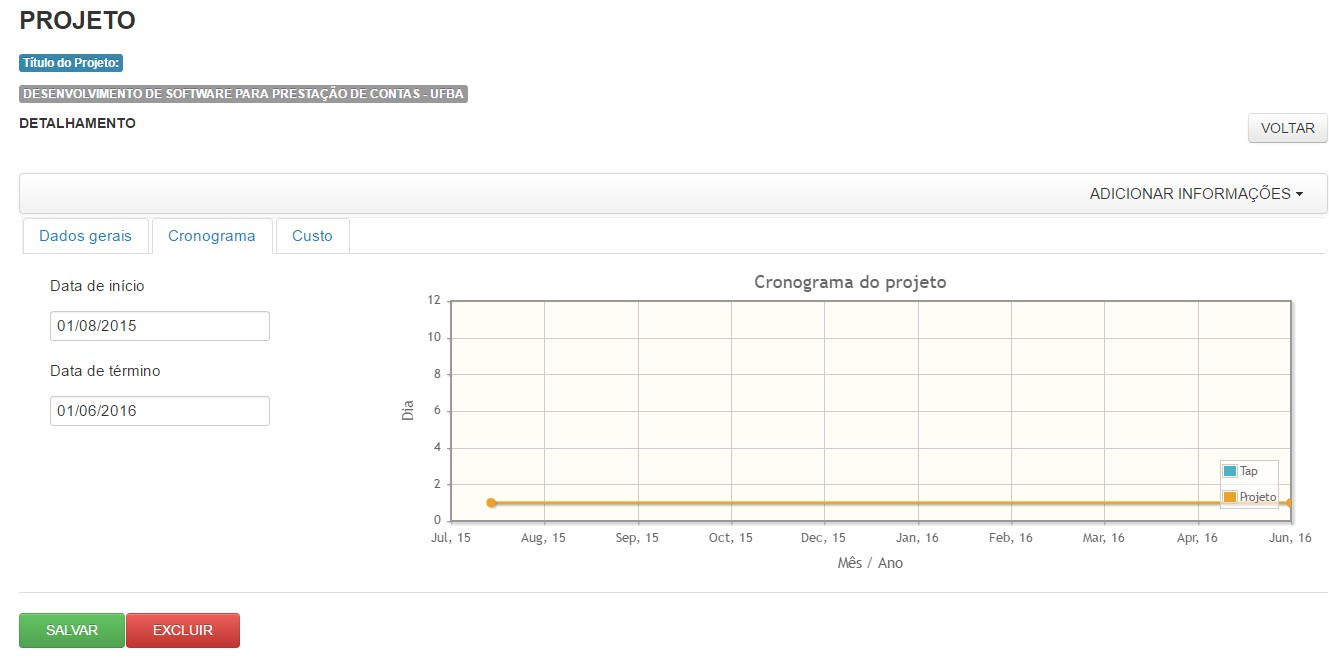
\includegraphics[width=0.5\textwidth]{RF_detalhamento_Projeto_Cronograma.jpg} % leia abaixo
\caption{Detalhes de um projeto cadastrado no sistema em função do seu cronograma de execução}
\end{figure}

\begin{figure}[h]
\centering % para centralizarmos a figura
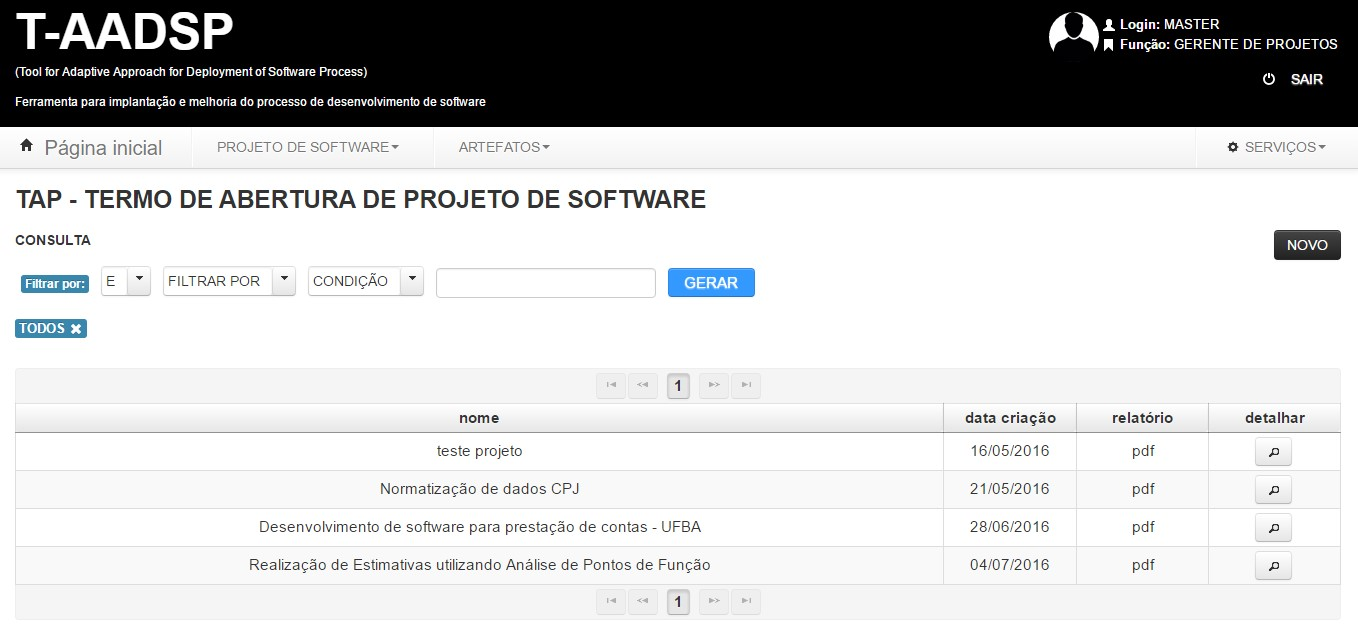
\includegraphics[width=0.5\textwidth]{RF_TAPConsulta.jpg} % leia abaixo
\caption{Consulta aos termos de abertura de projetos de software no sistema}
\end{figure}

\begin{figure}[h]
\centering % para centralizarmos a figura
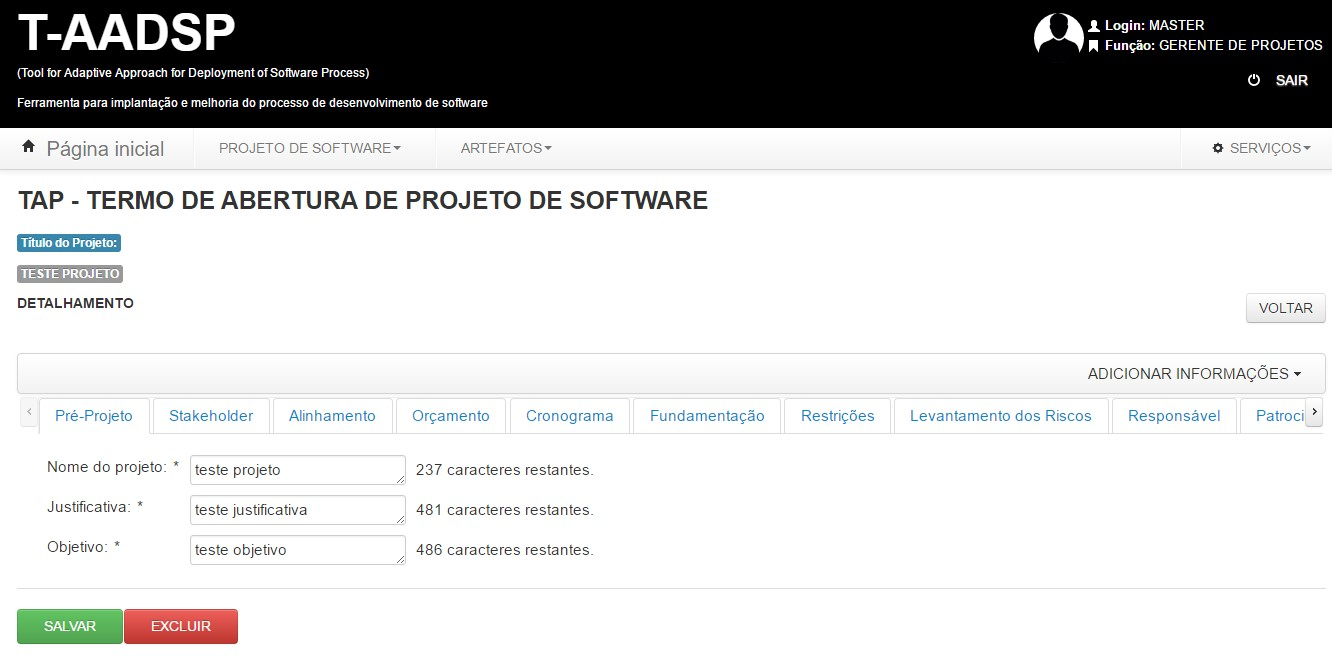
\includegraphics[width=0.5\textwidth]{RF_TAPDetalhamento.jpg} % leia abaixo
\caption{Detalhamento de um termo de abertura de projeto de software no sistema}
\end{figure}

\begin{figure}[h]
\centering % para centralizarmos a figura
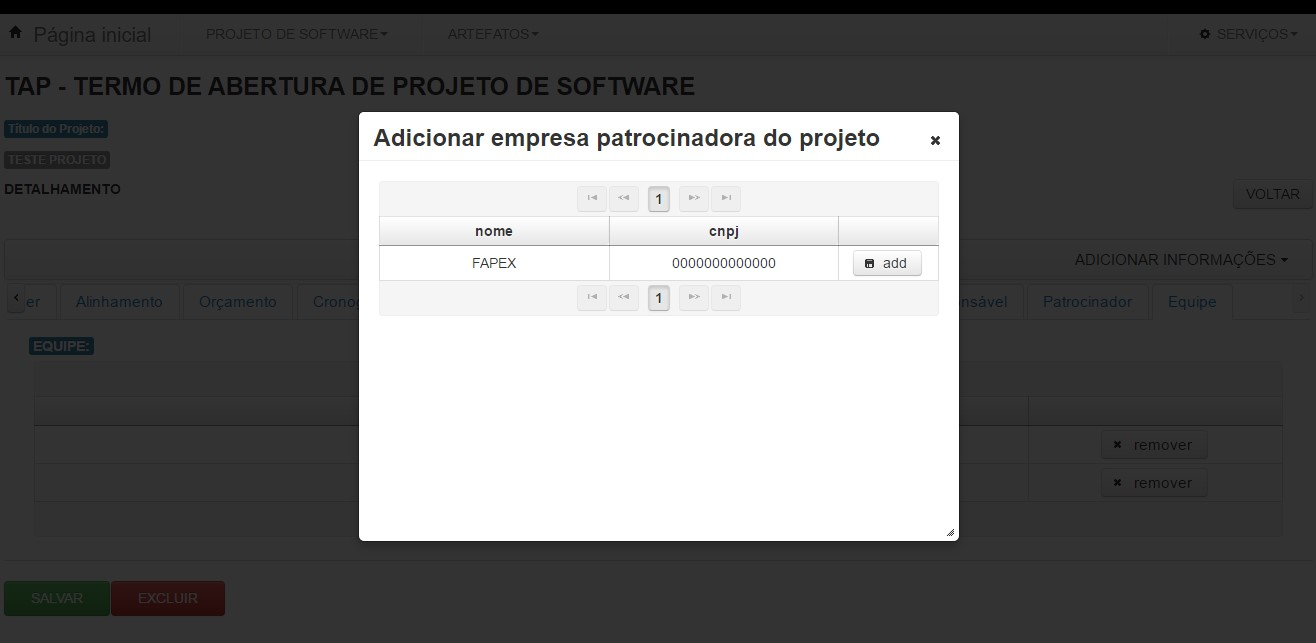
\includegraphics[width=0.5\textwidth]{RF_TAPDetalhamento_addPatrocinador.jpg} % leia abaixo
\caption{TAP: consulta aos patrocinadores de um projeto}
\end{figure}

\begin{figure}[h]
\centering % para centralizarmos a figura
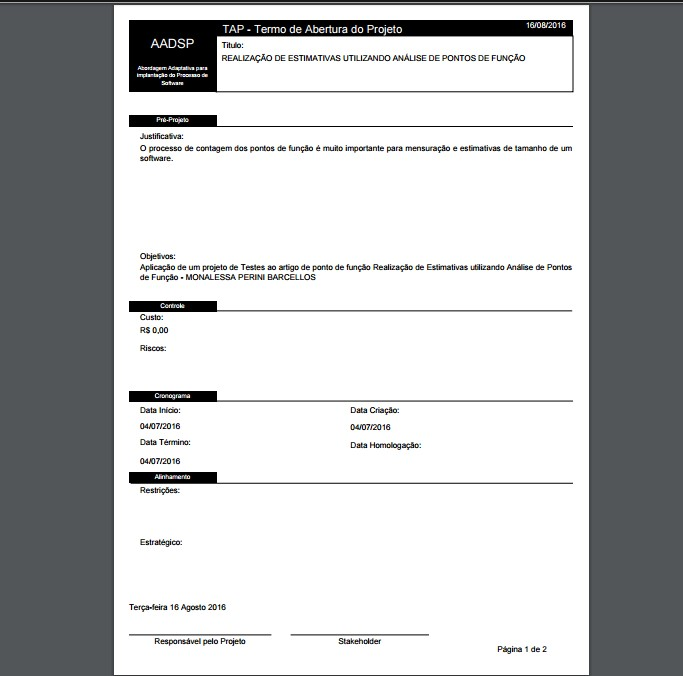
\includegraphics[width=0.5\textwidth]{RF_Termo_de_Abertura_de_projeto_em_PDF.jpg} % leia abaixo
\caption{TAP: em formato PDF}
\end{figure}


\begin{figure}[h]
\centering % para centralizarmos a figura
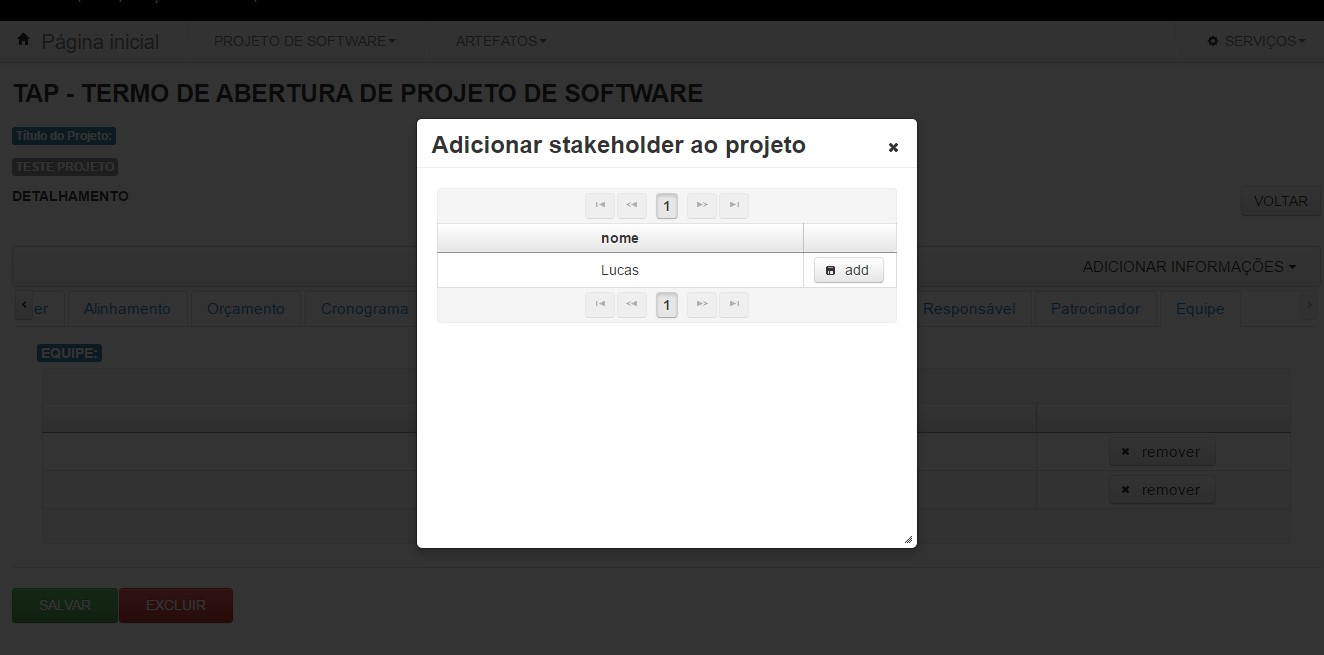
\includegraphics[width=0.5\textwidth]{RF_TAPDetalhamento_stakeholder.jpg} % leia abaixo
\caption{Consulta dos stakeholders do projeto}
\end{figure}

\begin{figure}[h]
\centering % para centralizarmos a figura
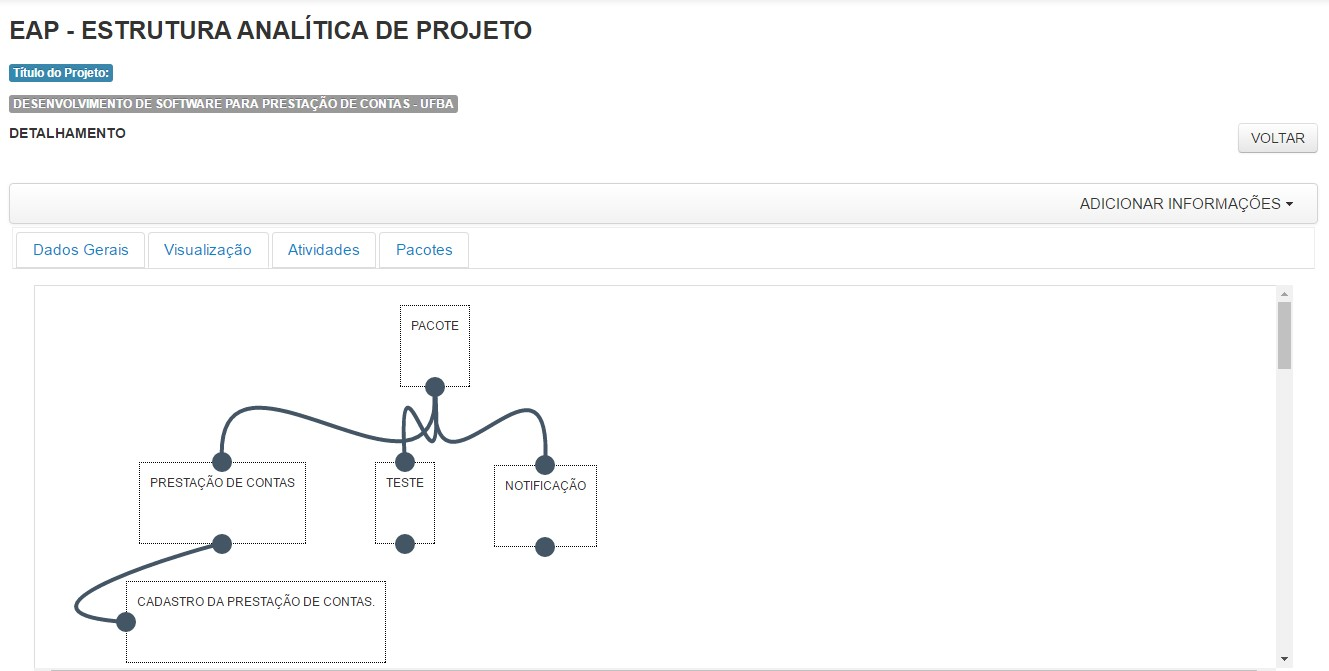
\includegraphics[width=0.5\textwidth]{RF_Eap_do_projeto_de_software.jpg} % leia abaixo
\caption{Estrutura analítica de um projeto e software}
\end{figure}

\begin{figure}[h]
\centering % para centralizarmos a figura
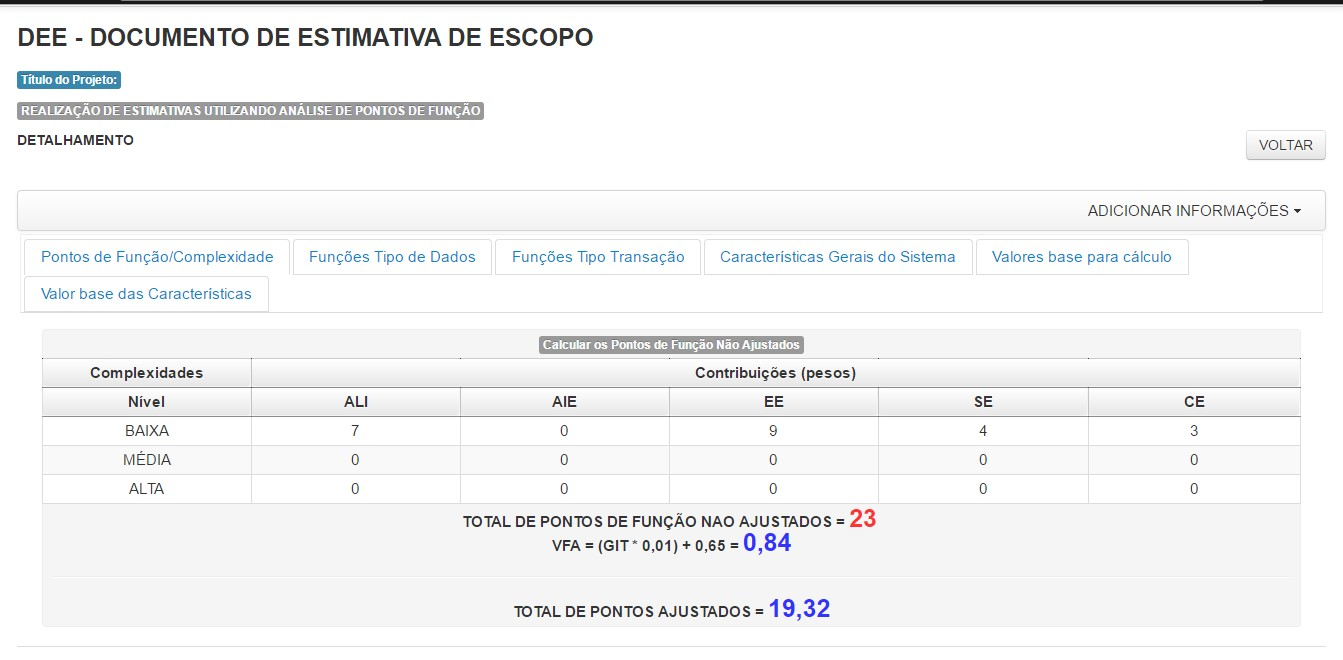
\includegraphics[width=0.5\textwidth]{RF_documento_de_estimativa_de_escopo.jpg} % leia abaixo
\caption{Documento de estimativa de escopo de um projeto - Cálculo dos pontos de função}
\end{figure}

\begin{figure}[h]
\centering % para centralizarmos a figura
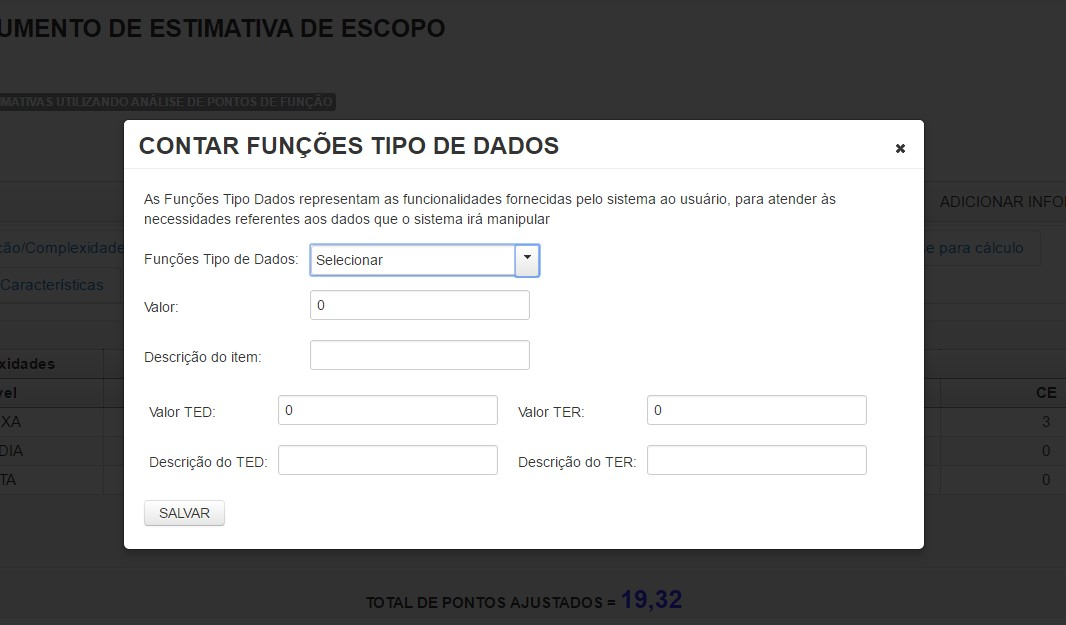
\includegraphics[width=0.5\textwidth]{RF_funcoes_tipos_de_dados_estimativa_de_escopo.jpg} % leia abaixo
\caption{Cálculo dos pontos de função: cadastro de funções de tipos de dados}
\end{figure}

\begin{figure}[h]
\centering % para centralizarmos a figura
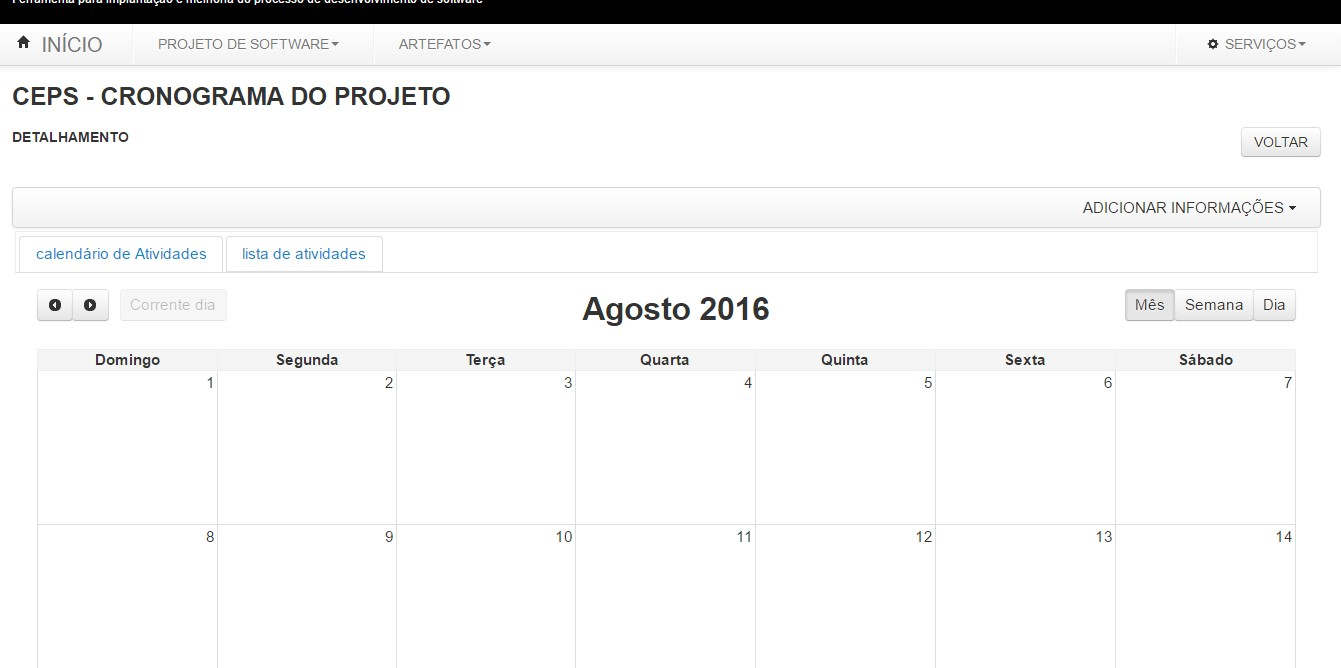
\includegraphics[width=0.5\textwidth]{RF_quadro_de_atividades_do_projeto.jpg} % leia abaixo
\caption{Calendário de atividades do projeto de software}
\end{figure}

\begin{figure}[h]
\centering % para centralizarmos a figura
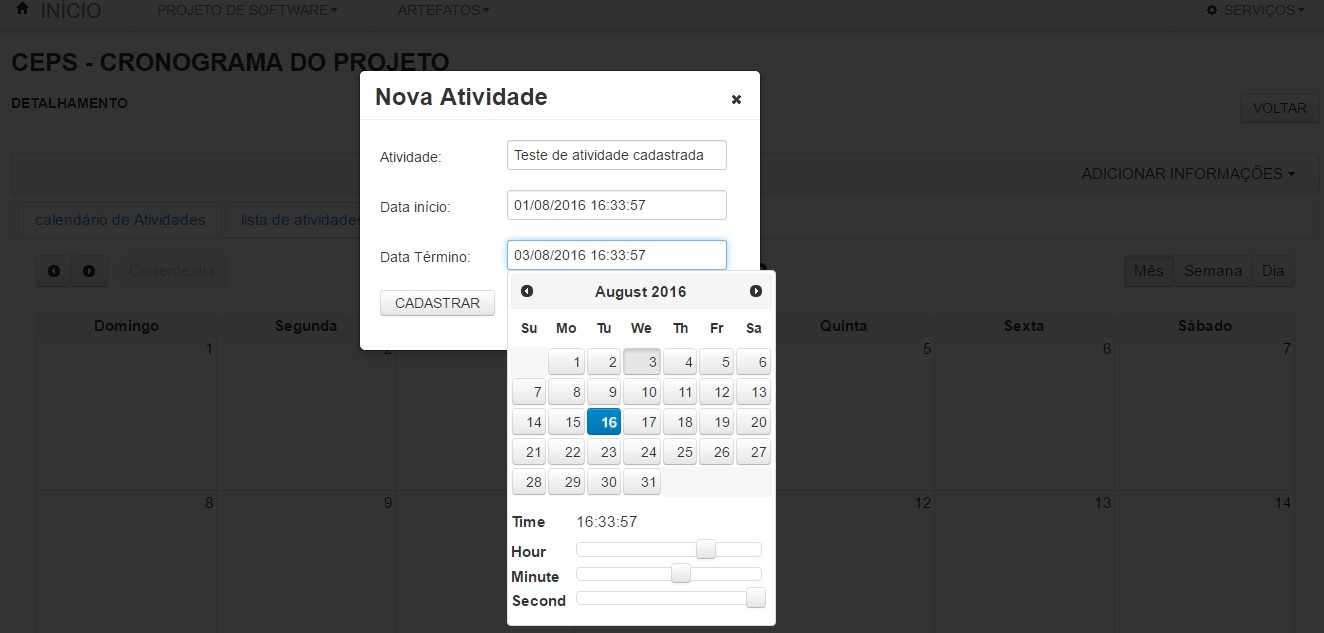
\includegraphics[width=0.5\textwidth]{RF_cadastr_de_atividade_para_projeto.jpg} % leia abaixo
\caption{Cadastro de atividades do projeto}
\end{figure}

\begin{figure}[h]
\centering % para centralizarmos a figura
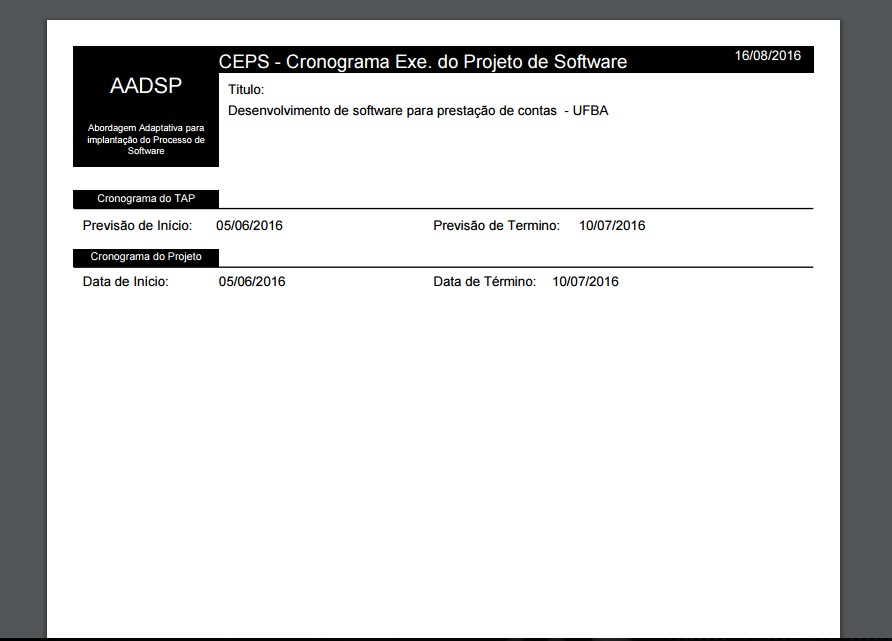
\includegraphics[width=0.5\textwidth]{RF_cronograma_do_projeto_PDF.jpg} % leia abaixo
\caption{Cronograma do projeto em formato PDF}
\end{figure}

\begin{figure}[h]
\centering % para centralizarmos a figura
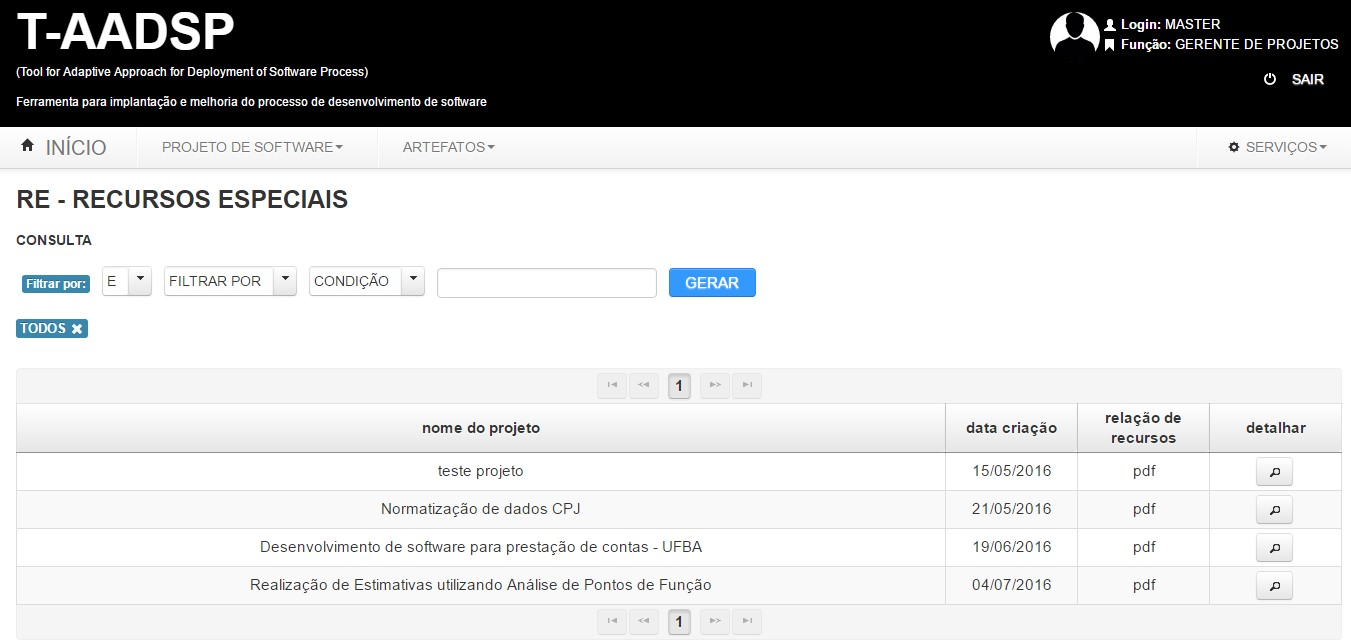
\includegraphics[width=0.5\textwidth]{RF_recursos_especiais_do_projeto.jpg} % leia abaixo
\caption{Cadastro de recursos do projeto}
\end{figure}

\begin{figure}[h]
\centering % para centralizarmos a figura
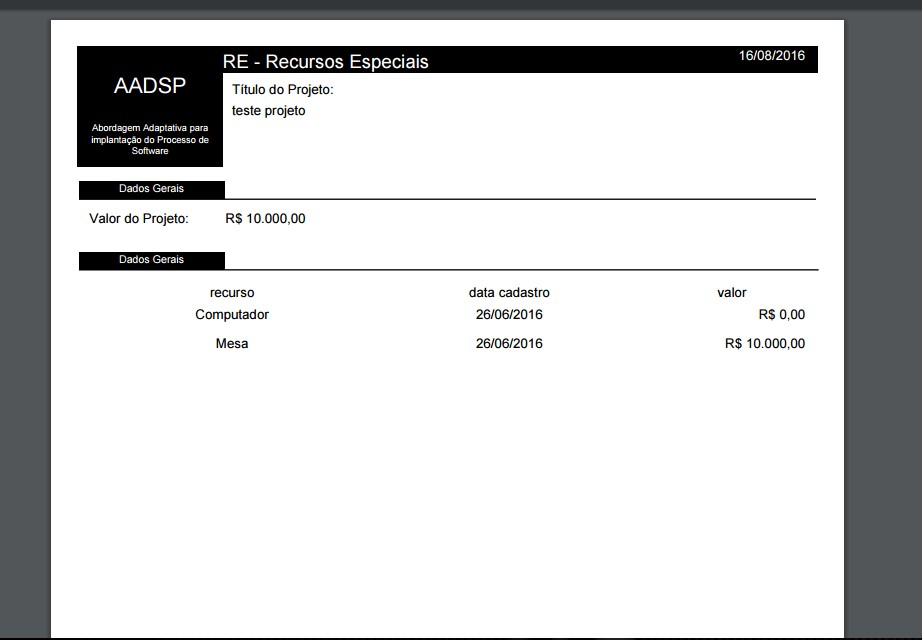
\includegraphics[width=0.5\textwidth]{RF_recursos_especiais_do_projeto_em_PDF.jpg} % leia abaixo
\caption{Lista dos recursos especiais do projeto em formato PDF}
\end{figure}



% documento de estimativa de escopo %

\begin{figure}[h]
\centering % para centralizarmos a figura
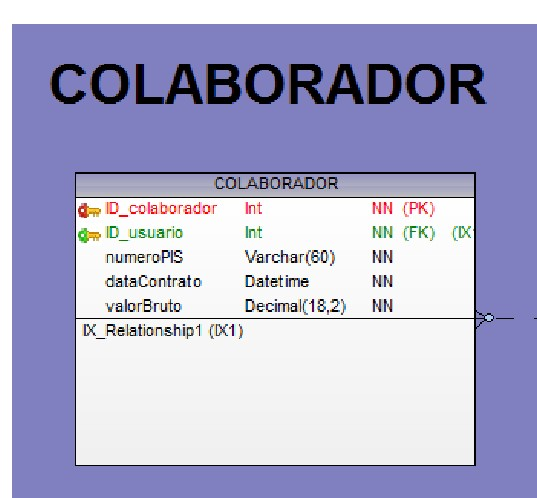
\includegraphics[width=0.5\textwidth]{DER_colaborador.jpg} % leia abaixo
\caption{Diagrama de Entidade e Relacionamento - Schema Colaborador}
\end{figure}

\begin{figure}[h]
\centering % para centralizarmos a figura
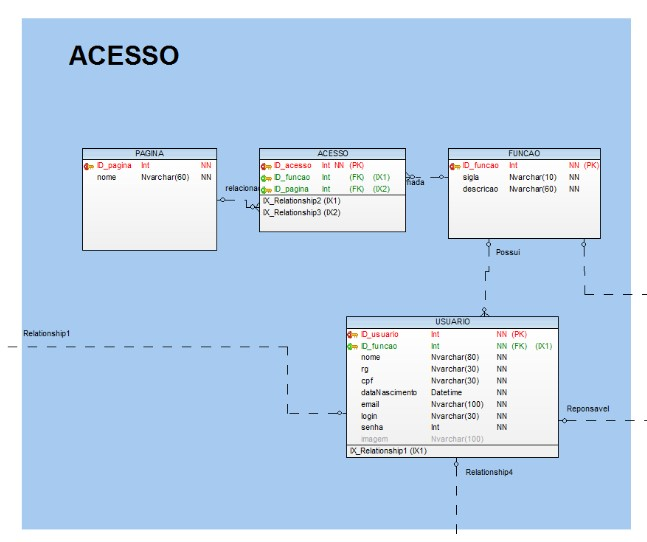
\includegraphics[width=0.5\textwidth]{DER_acesso.jpg} % leia abaixo
\caption{Diagrama de Entidade e Relacionamento - Schema Acesso}
\end{figure} 

\begin{figure}[h]
\centering % para centralizarmos a figura
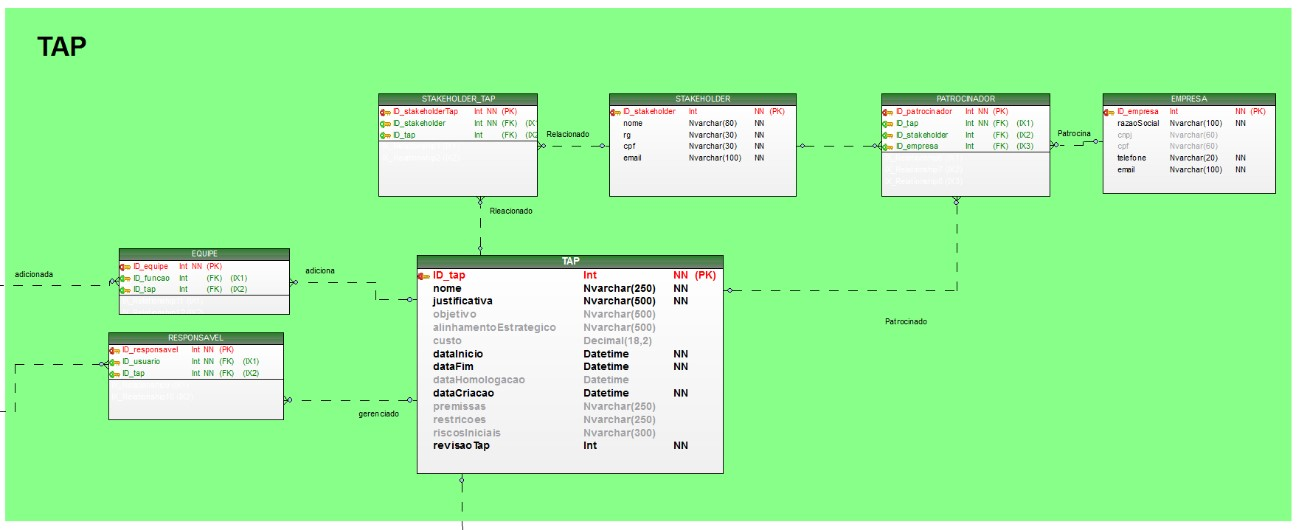
\includegraphics[width=0.5\textwidth]{DER_tap.jpg} % leia abaixo
\caption{Diagrama de Entidade e Relacionamento - Schema Tap}
\end{figure}

\begin{figure*}[h]
\centering % para centralizarmos a figura
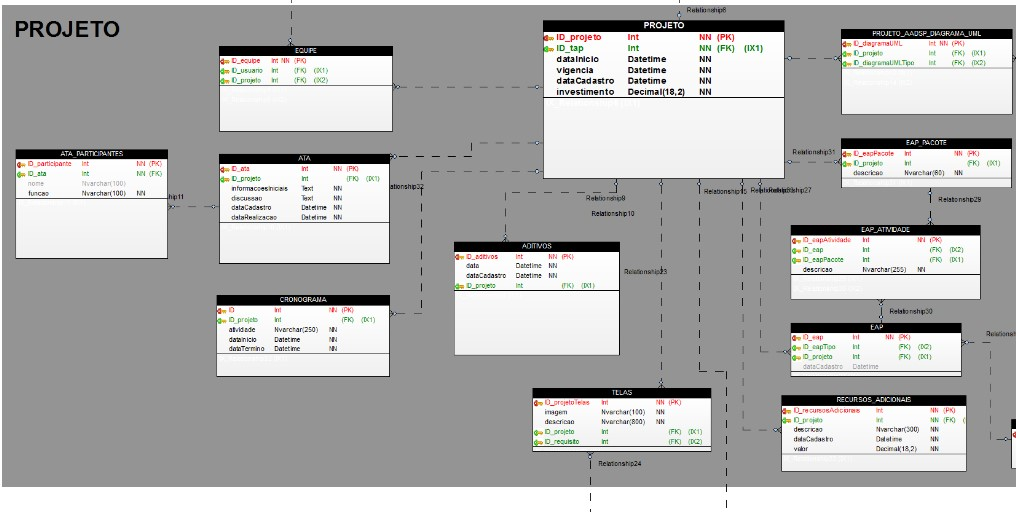
\includegraphics[width=1\textwidth]{DER_projeto_p1.jpg} % leia abaixo
\caption{Diagrama de Entidade e Relacionamento - Schema Projeto Parte 1}
\end{figure*}

\begin{figure*}[h]
\centering % para centralizarmos a figura
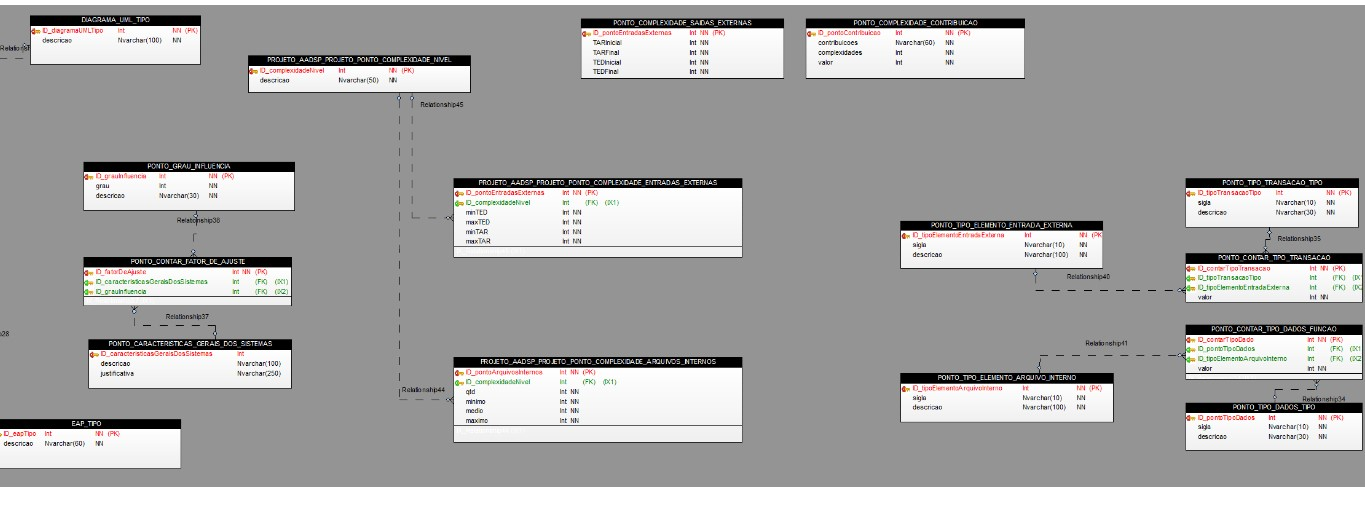
\includegraphics[width=1\textwidth]{DER_projeto_p2.jpg} % leia abaixo
\caption{Diagrama de Entidade e Relacionamento - Schema Projeto Parte 2}
\end{figure*}


\end{appendices}

\end{document}
